

\documentclass[a4paper,11pt]{article}
\usepackage[utf8]{inputenc}
\usepackage[T1]{fontenc}
\usepackage{amsmath,amssymb}
\usepackage{mathtools}
\usepackage{algorithm}
\usepackage{algorithmicx}
\usepackage{algpseudocode}
\usepackage{float}
\usepackage{xcolor}
\usepackage{url}
\usepackage{booktabs}
\usepackage{graphicx}
\usepackage{tikz}
\usepackage{siunitx}
\usepackage[margin=0.8in]{geometry}

\usepackage{authblk}
\title{How do you choose the best MEV strategy?}
\author[1]{Daniele Maria Di Nosse\textsuperscript{\dag}}
% \author[1]{Fabrizio Lillo}

\affil[1]{Scuola Normale Superiore, Pisa, Italy}
\date{\today}

\begin{document}

\maketitle
\begin{center}
  \footnotesize
  \dag Corresponding author. Email: \texttt{daniele.dinosse@sns.it}
\end{center}
\begin{abstract}
Maximal extractable value (MEV) arises when transaction ordering around user swaps can be exploited. We develop a simple Uniswap v3 framework that compares the profitability of back-running arbitrage, sandwich attacks, just-in-time (JIT) liquidity provision, and a mixed JIT+sandwich bundle as a function of swap size, fee tier, and slippage tolerance. Under a single-tick approximation we derive profit ceilings (hence bribe bounds) and show that slippage constraints cap the optimal front-run, generating sharp regime transitions: for swaps below a fee-scale threshold the optimal bundle is pure JIT, while above it mixed strategies can dominate, especially in higher-fee pools. Using on-chain data from the USDC--WETH 0.05\% pool in 2023, we find qualitative agreement with these regimes and deviations consistent with cross-tick execution and non-optimal parameter choices.
\end{abstract}
% TODO: talk about OFAC-regulated relays (mevwatch.info)
\section{Introduction}
\label{sec:mev}

Decentralized exchanges (DEXs) such as Uniswap v3 \cite{adams2021} settle trades through deterministic smart contracts. The public nature of execution---transactions are visible before inclusion and are executed atomically within blocks---creates opportunities to profit from \emph{transaction ordering} rather than from directional bets. The additional value that can be extracted by inserting, reordering, or censoring transactions around a user swap is known as maximal extractable value (MEV)\footnote{The term was originally introduced as \emph{miner extractable value}; see \cite{flashboys}.}.

This paper studies MEV around large swaps in Uniswap v3. We focus on four canonical patterns observed in practice: back-running arbitrage, sandwich attacks, just-in-time (JIT) liquidity provision, and a mixed JIT+sandwich construction. Under a single-tick approximation of Uniswap v3, we derive simple profit expressions that clarify how profitability scales with the fee tier, the user’s slippage tolerance, and the swap size. Throughout, we interpret these profits as upper bounds on the bribes an MEV searcher can rationally pay for inclusion while remaining profitable.

MEV, however, is not solely a ``mempool'' phenomenon: modern Ethereum execution is mediated by specialized actors (searchers, builders, relays, and validators) and increasingly by private order-flow channels. The next subsection summarizes the Proposer--Builder Separation (PBS) pipeline and introduces the payoff notation used in the rest of the paper.

\subsection{Proposer-Builder Separation (PBS)}
In traditional electronic markets, orders are matched nearly continuously and the main microstructure frictions are latency and queue priority. On Ethereum, transactions are executed in discrete blocks (12-second slots): after submission they propagate through nodes and sit in a memory pool (\textit{mempool}) until included by a validator. Because the public mempool reveals the full contents of pending transactions, the impact of a large swap on an AMM can be simulated before it executes. This makes the interval between submission and inclusion the natural arena where MEV strategies are constructed.

When competition takes place in the public mempool, searchers can bid for priority by paying higher gas tips, leading to priority-gas auctions (PGAs) and potentially higher costs for ordinary users.\footnote{Under EIP-1559 the transaction fee is split into a base fee (burned) and a priority fee (paid to the block producer).} Proposer--Builder Separation (PBS) was proposed to reduce these externalities and to mitigate incentives for validators to vertically integrate the block-building function \cite{buterinPBS2021}. PBS separates the \textit{proposer} role (consensus: choosing a block to sign) from the \textit{builder} role (execution: constructing the block payload and ordering transactions). While PBS is currently implemented through third-party infrastructure, protocol-level designs remain an active research direction \cite{ethereumPBS2024}.

The most widely adopted implementation is Flashbots' MEV-Boost (\url{https://boost.flashbots.net/}) \cite{mevboost_pics}. Searchers submit (atomic) bundles and bids to builders; builders assemble candidate blocks and forward only headers and bids to trusted intermediaries known as \textit{relays}. Proposers query relays for their best-paying header, sign the highest bid, and only then receive the full block. Figure~\ref{fig:pbs_schema} summarizes this flow (see \cite{oz2024wins} for a detailed account). Off-chain auctions reduce the need for public gas bidding, but they also concentrate power in a small set of professional builders/relays and create additional points where failures or policy-driven filtering can affect execution \cite{marzecThibault2024,damatoNeuder2023}.

\begin{figure}
    \centering
    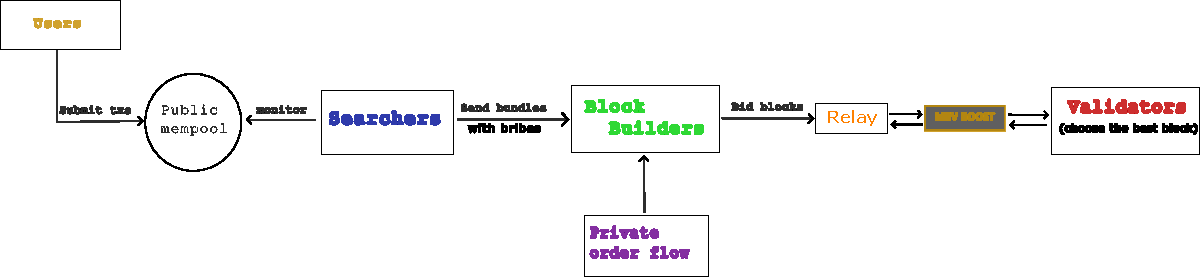
\includegraphics[width=0.8\linewidth]{figures_st_app/pbs.pdf}
    \caption{PBS schema}
    \label{fig:pbs_schema}
\end{figure}
In parallel with PBS, an increasing share of high-value transactions bypasses the public mempool. Wallets and bots may submit transactions directly to builders via private RPC endpoints or order-flow auctions, creating \textit{exclusive order flow} (EOF). EOF reduces exposure to mempool-based attacks for the sender, but gives builders a first (sometimes exclusive) look at the trade and changes the bargaining over who captures MEV.\footnote{In some arrangements the builder is explicitly allowed to insert complementary transactions (e.g., back-runs) around the private order.} Depending on the channel, part of the extracted MEV may be rebated to the sender, or the sender may pay for protection against adverse ordering (e.g., sandwiching).

Overall, PBS turns MEV into an explicit market for inclusion and ordering, with bids and side-payments complementing gas fees. Figure~\ref{fig:historical_gasprice} shows the historical dispersion of gas prices (min/max within each block), a footprint of the intensity of competition for priority.

\begin{figure}
    \centering
    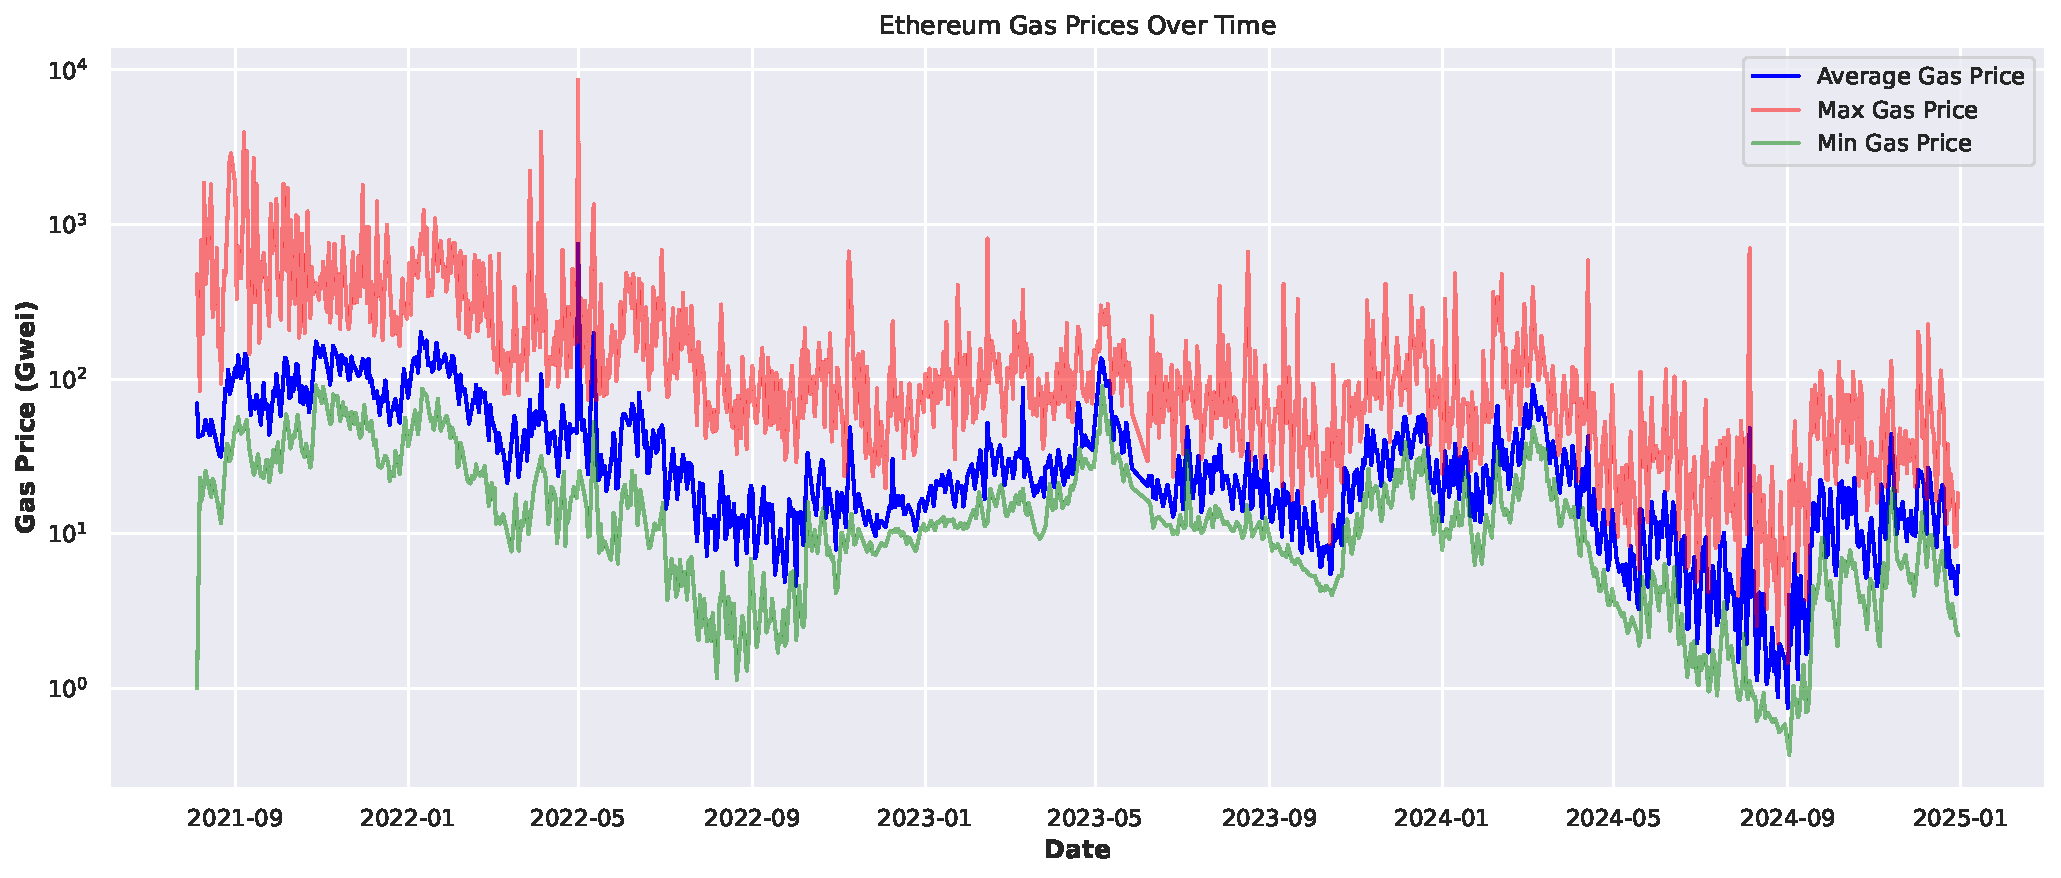
\includegraphics[width=0.8\linewidth]{figures_st_app/historical_gas_prices.pdf}
    \caption{Hiastorical gas price from 05/08/2021 (first available day of the DexGuru Ethereum Gas Tracker) to 31/12/2024. The Min Gas Price represents the lowest fee paid for a transaction to be included in a block, while the Max Gas Price is the highest fee paid in that same block — reflecting the range of urgency and cost users were willing to pay. }
    \label{fig:historical_gasprice}
\end{figure}
\vspace{1em}

To fix notation for the rest of the paper, we decompose the per-block profits of the three main actors (searchers, builders, and validators) as follows:

%-----------------------------------------------------------------------
% 2 Profit functions
%-----------------------------------------------------------------------
%----------------------------------------------------------
% Profit functions (ETH units, per block)
%----------------------------------------------------------
\begin{align}
\textbf{Searcher:}\quad
\pi_s &= M
        -\bigl(
            C_{\text{gas}}
          + D_{\text{sb}}
          + C_{s,\text{infra}}
        \bigr) \\[6pt]
%
\textbf{Builder:}\quad
\pi_b &= R
        - \bigl(1+\rho\bigr)B   % bid paid to validator plus relay fee
        - R_{\text{refund}}     % on-chain user rebate
        - C_{b,\text{infra}} \\[6pt]
%
\textbf{Validator:}\quad
\pi_v &= B
        + R_{\text{consensus}}
        - C_{v,\text{infra}}
\end{align}

%----------------------------------------------------------
% Refund calculus (inside the same block)
%----------------------------------------------------------
\[
   R_{\text{refund}}
      \;=\; \varphi\,D_{\text{sb}},\qquad
   0\le \varphi \le 1.
\]

%----------------------------------------------------------
% Raw block value (unchanged from the papers)
%----------------------------------------------------------
\[
  R = \sum_{i\in\text{tx}}
        \bigl(
          \text{priority fee}_i
          + \text{direct transfer}_i
        \bigr).
\]

%----------------------------------------------------------
% Symbol glossary (additions in blue)
%----------------------------------------------------------
\begin{center}
\begin{tabular}{@{}ll@{}}
\toprule
Symbol & Meaning \\ \midrule
$R$ & Raw block value (priority-fee tips $+$ direct transfers) \\
$B$ & Builder\,$\to$\,proposer payment (coinbase transfer) \\
$M$ & MEV revenue realised in the searcher’s bundle(s) \\
$C_{\text{gas}}$ & Gas actually paid by the searcher’s bundle \\
$D_{\text{sb}}$ & Direct ETH transfer (tip) from searcher to builder \\
$\varphi$ & Refund ratio ($0\!-\!1$) set by MEV-Share or similar \\
$R_{\text{refund}}$ & On-chain rebate to user: $\varphi D_{\text{sb}}$ \\
$\rho$ & Relay-fee fraction on the builder’s bid ($0\!-\!1$) \\
$C_{s,\text{infra}}$ & Off-chain infrastructure costs of the searcher \\
$C_{b,\text{infra}}$ & Builder infrastructure \& order-flow costs \\
$C_{v,\text{infra}}$ & Validator infrastructure costs \\
$R_{\text{consensus}}$ & Protocol-level block-proposal reward \\ \bottomrule
\end{tabular}
\end{center}


% where $\text{refund}_b$ is the portion of the value a bundle generates that is explicitly routed back to the original order-flow owner (the user, wallet, or dApp that sent the protected transaction).
% It only appears when the bundle travels through an Order-Flow Auction (OFA) such as Flashbots Protect / MEV-Share or MEV-Blocker.
% In those channels the user agrees to share enough data about their transaction to let searchers back-run it, but on the condition that they receive a preset share of whatever MEV is realised
% \[
% \begin{aligned}
% \Pi_{\text{searcher}}
% &=
% \sum_{b \in \text{bundles}}
% \Bigl(
% \underbrace{\Delta\mathrm{state}_{b}}_{\substack{\text{value extracted}\\\text{by the searcher}}}
% \;-\;
% \underbrace{\mathrm{gas}_{b}}_{\substack{\text{gas fees}\\\text{paid on-chain}}}
% \;-\;
% \underbrace{\mathrm{bribe}_{b}}_{\substack{\text{priority-fees or}\\\text{coinbase tips to builder}}}
% \;-\;
% \underbrace{\mathrm{refund}_{b}}_{\substack{\text{any rebate or}\\\text{OFA refund paid}}}
% \Bigr)
% \\[1em]
% \Pi_{\text{builder}}
% &=
% \underbrace{v_{\text{true}}}_{\substack{\displaystyle\sum_{i}\bigl(\mathrm{tip}_{i}+\mathrm{cb}_{i}-\mathrm{refund}_{i}\bigr)\\\text{(total block value)}}}
% \;-\;
% \underbrace{(1+\rho)\,\mathrm{bid}}_{\substack{\text{payment to proposer}\\\text{plus relay fee}}}
% \\[1em]
% \Pi_{\text{validator}}
% &=
% \underbrace{\mathrm{bid}}_{\text{builder→proposer payment}}
% \;+\;
% \underbrace{\gamma\sum_{i}\mathrm{tip}_{i}}_{\substack{\text{priority fees}\\\text{from each tx}}}
% \;+\;
% \underbrace{\mathrm{issuance}}_{\substack{\text{staking rewards}\\\text{(new ETH minted)}}}
% \;-\;
% \underbrace{\mathrm{penalties}}_{\substack{\text{slash fines or}\\\text{missed duties}}}
% \end{aligned}
% \]
\begin{figure}
    \centering
    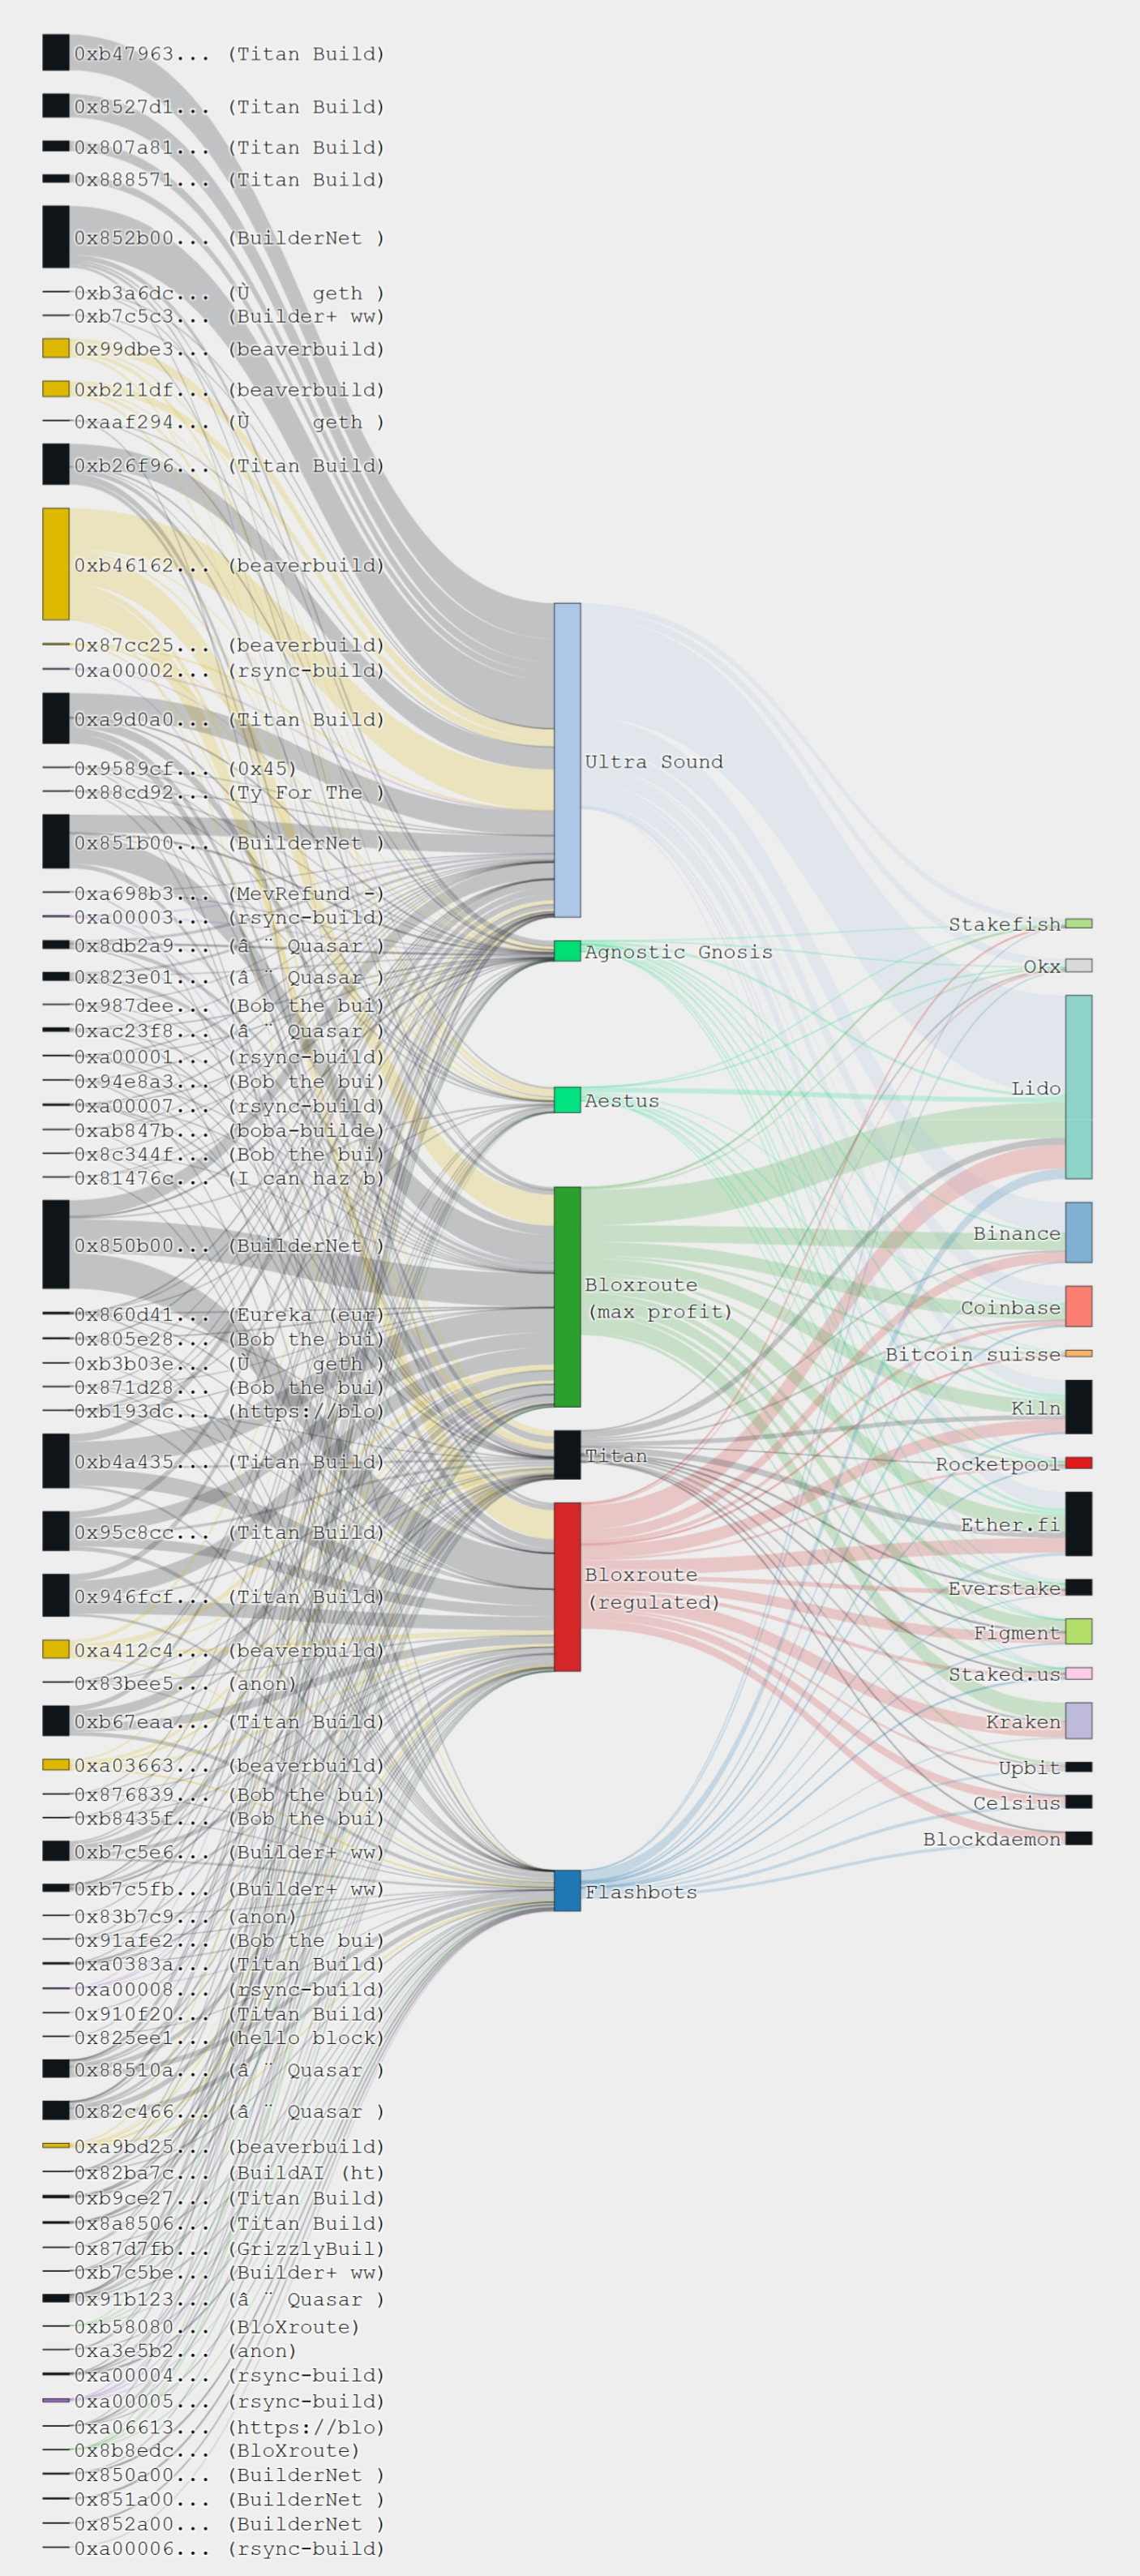
\includegraphics[width=0.5\linewidth]{figures_st_app/blockbuilder_relay_validator.png}
    \caption{Caption}
    \label{fig:builder_relay_validator}
\end{figure}

\paragraph{Paper organization.}
The remainder of Section 2 presents the main MEV strategies and their closest analogues in traditional finance. Section 3 derives profit expressions for JIT liquidity provision, back-running arbitrage, sandwich attacks, and a mixed JIT+sandwich strategy in Uniswap v3, and interprets these profits as bounds on feasible bribes. Section 4 compares these theoretical predictions with realized on-chain profits for the USDC--WETH 0.05\% pool in 2023. Appendix A collects tick-aware execution rules for Uniswap v3 that relax the single-tick approximation used in the main text.
\subsection{MEV/Manipulation Strategies}
In this section we present  a narrative that walks through different MEV strategies and carefully draws parallels to its closest equivalent in traditional finance (TradFi), unpacking how each tactic works, what the motivations are, and where the two domains differ due to rules, infrastructure, or ethics. 
We will focus on the most widely used strategies \footnote{For a comprehensive survey about MEV in DeFi, see \cite{materwala2024maximal}.}. They include arbitrages, sandwich attacks and Just-in-Time liquidity. 

\subsubsection{Flash--loan attacks}
\label{subsec:flashloans}

A flash loan allows any Ethereum user to borrow  an arbitrary amount of ERC-20 liquidity without any kind of collateral provided that the entire borrow $\rightarrow$ exploit $\rightarrow$ repay sequence is executed atomically inside a single transaction.  This means that the lender’s solvency risk is zero (the call reverts if the repayment fails). All the strategies described below can (and actually do) include a flash loan as initial step. Indeed, a meta-study of the 100 largest DeFi hacks through 2024 finds that roughly
60\% of all price-manipulation exploits relied on flash loans
\cite{halborn2024survey}. In addition, flash loans can also be used to perform hijack on governance-tokens based protocols, like Decentralized Autonomous Organizations (DAOs). In this case, the attacker flash-borrow $>$51\,\% of a token supply, pass a malicious proposal in the same transaction, drain the treasury, and repay.

There is no analogue of unlimited, unsecured and atomic credit in TradFi.

\subsubsection{Arbitrage}
In these cases, MEV searchers can exploit price mismatches between two pools, two DEXs or even DEX and CEX. In such a way, they contribute to market efficiency. We can distinguish between atomic arbitrages and non-atomic arbitrages. The first ones involve only on-chain operations and are executed using atomic transactions to buy the cheaper asset and simultaneously sell the more expensive one, usually within a single block. Furthermore, thanks to the atomicity of smart contracts, the searcher can also take advantage of flash loans \footnote{A flash loan on Ethereum is a type of unsecured loan offered by certain decentralized finance (DeFi) protocols (e.g., Aave or dYdX) that allows users to borrow assets instantly and without collateral, as long as the loan is repaid within the same blockchain transaction} to perform the strategy without upfront capital. It is therefore an almost riskless strategy since if the transaction fails, the searcher only loses the gas fee paid. Instead, non-atomic arbitrages refer to DEX-CEX arbitrages, where the searcher must interact with an off-chain platform (the CEX) and so she cannot exploit the atomicity of the smart contracts, exposing herself to the risk of a non-profitable arbitrage due to adverse price movements before the validation of her transactions.

What we have just described can be labeled as beneficial for the market, since it helps the information flows trough the different market venues in the DeFi ecosystem. However, it is important to note that there are some malicious types of arbitrage that can be called 'price manipulation arbitrages'. In this scenario, a user takes a flash loan, uses part of it to borrow a token (like WBTC) on a lending platform, and another part to execute a leveraged trade that pushes up the token’s price on a low-liquidity AMM. They then sell the borrowed tokens at the inflated price and repay the flash loan, keeping the profit. All of this is possible due to smart contract bugs being exploited.

In order to understand this dynamics, it can be helpful to illustrate one famous example of this attack. It happened in 2020 on the protocol bZx. In that case, the attacker did exactly what we have already discussed: he took a flash loan of 10,000 ETH and used 5,500 ETH as collateral on Compound to borrow 112 WBTC, while using 1,300 ETH to open a 5x leveraged margin trade on bZx. The margin trade routed through Kyber and executed a large ETH-to-WBTC swap on Uniswap, which had low liquidity at the time. This trade itself caused the price of WBTC to spike from around 38 ETH to over 109 ETH. Due to a bug in the bZx smart contract, the system failed to perform a proper collateralization check after the trade and accepted the manipulated price as valid. As a result, the attacker was able to sell the 112 borrowed WBTC for 6,871 ETH, repay the 10,000 ETH flash loan, and walk away with a net profit of around 1,271 ETH, worth approximately \$355,000 at the time, leaving the protocol with bad debt.

In traditional finance, this maps closely to multi-venue arbitrage, a classic strategy in equity and FX markets. High-frequency trading (HFT) firms monitor multiple exchanges using direct, ultra-low-latency data feeds. When they detect a stale price on one venue they race to buy low and sell high before the prices converge. Similar strategies are used between ETFs and their underlying baskets.

Key differences:
\begin{itemize}
    \item In TradFi, trades are not atomic—there’s real execution and inventory risk during the latency window.
    % \item Under MiFID II’s best-execution mandate—enforced in Italy by CONSOB—brokers must seek the best possible result across Borsa Italiana, MTFs and systematic internalisers, effectively delivering an NBBO-like outcome for Italian investors.
    \item in TradFi infrastructure is a huge barrier: collocation, proprietary data feeds, and microwave networks can cost tens of millions annually.
    \item In DeFi, a simple Ethereum transaction with the right logic can do the same work for a few dollars in gas.
\end{itemize}

% \subsubsection{Liquidations}
% DeFi lending protocols like Aave or MakerDAO allow anyone to liquidate under-collateralized positions by repaying part of the borrower’s debt and receiving a discounted portion of their collateral. This happens automatically as soon as the loan-to-value (LTV) ratio breaches a set threshold, and liquidators (MEV searcher) compete openly to be the first to act.

% In TradFi, this parallels margin calls and default liquidations in brokerage and derivatives markets. When an investor’s equity drops below the maintenance margin, their broker issues a margin call. If not met within a specific timeframe, the broker forcibly liquidates their position—usually via smart-order routing that seeks best execution. In futures markets, clearinghouses like CME organize default auctions where member firms bid to take over the risk of failing counterparties. Repo markets do similar things via General Collateral Finance (GCF) auctions.

% Key differences:
% \begin{itemize}
%     \item TradFi liquidations are centrally managed by brokers or clearinghouses, with best-execution obligations and reporting duties (e.g., Form 1099-B in the U.S.).
%     \item DeFi liquidations are decentralized and public: any address can try, and speed is determined by gas and mempool positioning.
%     \item TradFi gives borrowers time to cure margin violations. DeFi executes the liquidation in the very same block that LTV fails.
% \end{itemize}

\subsubsection{Sandwich attacks}
Sandwich attacks are strategies designed for gaining from the price impact of a large swap (performed by the victim) pending in the mempool. The MEV searcher acts as follows. Firstly, a swap is placed in the same direction as the victim (also known as front run); then, the victim swap is executed \footnote{There is of course the possibility of multiple victims' swaps}; lastly, the attacker closes the position by placing a swap with the same amount and opposite sign to the front run (also known as back run). This type of attack harms market participants, as the victim pays a higher price due to the impact of the front run swap.

The victim can protect herself from this type of attack by setting a low slippage tolerance on her transaction. This means that if the swap would result in receiving less than a certain minimum amount, the transaction will automatically fail. As a result, the attacker must carefully choose how much to front-run—if they push the price too far, the victim’s transaction will not go through, and the attack fails.

The TradFi analogue is front-running, either in its classic form (e.g., a broker trading ahead of a client order) or in more modern, legal gray zones like latency arbitrage. HFT firms use predictive models and "ping" orders to infer large institutional activity. If detected early, HFTs may quickly buy shares in one venue before the order hits and sell them at a slightly higher price moments later.

Key differences:
\begin{itemize}
    \item On Italian markets, dealing on non-public client information is prohibited by the EU Market Abuse Regulation (MAR) and Articles 184-187-ter of Italy’s Consolidated Finance Act (TUF), so front-running is a criminal behaviour.
    \item In DeFi, the mempool is public. This makes sandwich attacks legally murky: technically, the bot is acting on public data, not insider information.
    \item TradFi has surveillance systems, anti-internalization rules, and dark pool disclosures. DeFi is experimenting with privacy-preserving alternatives (e.g., encrypted mempools, SUAVE) but lacks formal enforcement.
\end{itemize}

\subsubsection{Just-in-Time (JIT) liquidity}
JIT liquidity is a strategy for gaining the fee that a large swap in the mempool will pay once executed. The MEV searcher deposits liquidity in a very narrow price range (containing the current price) just before the transaction is processed, earning most of the trading fee, and removes the liquidity immediately after the transaction. This strategy is also referred to as \textit{LP sandwich} or \textit{active liquidity provision}\footnote{Despite this definition is very appealing, it should not be confused with the so-called \textit{active liquidity}, that is the sum of all the liquidity whose range contains the price.} \cite{capponi2023paradox}, as the liquidity provision is elicited by a pending order in the mempool. The liquidity provider never intends to provide ongoing liquidity; they simply "ride" the trade. In contrast to sandwich attacks, JIT liquidity is beneficial for the end user due to the enhanced liquidity that lower the price impact of the swap.

In TradFi there is not a direct analogue of this strategy, but it resembles fleeting quotes and rebate-seeking behavior. On venues available to Italian firms, HFTs sometimes flash tight quotes on pan-European MTFs such as Cboe Europe CXE/BXE, which still rebate about 0.15 bps to passive fills. By contrast the main Euronext Milan order book merely waives or halves the passive fee rather than paying cash.
% Market makers also internalize retail flow only when conditions are favorable—like in payment-for-order-flow (PFOF) systems where brokers route trades to wholesalers who offer price improvement and liquidity only when profitable.

Key differences:
\begin{itemize}
    \item TradFi exchanges now limit these tactics. MiFID II empowers CONSOB and Borsa Italiana to impose order-to-trade-ratio caps and minimum quote-life parameters, preventing excessive 'quote flicker' by HFT algorithms.
    \item In Uniswap, there is no time-in-force constraint—adding and removing liquidity can happen in a single atomic transaction.
    \item TradFi rebates are paid by the venue; in DeFi, traders themselves pay LP fees. The design incentive is inverted.
\end{itemize}



\subsubsection{Mixed (Sandwich+JIT) attacks}
It is worth noting that the state-of-the-art to exploit a large swap in DeFi is a combination of JIT and Sandwich attacks. When a large swap is detected in the mempool, a mixing attack made up of a JIT encapsulated into a sandwich could sometimes bring the highest profit. Specifically, the exact scheme is: front run, mint liquidity, victim swap, burn liquidity, back run.\\


\noindent MEV strategies aren’t new—they are just smart-contract-powered expressions of long-standing financial instincts: arbitrage, front-running, fleeting liquidity provisioning etc. What sets DeFi apart is its:
\begin{itemize}
    \item \textbf{Atomicity}: execution is all-or-nothing in a single block
    \item \textbf{Transparency}: everything is visible (and exploitable) in the mempool.
    \item \textbf{Permissionlessness}: anyone with code and gas can participate—no licenses, no seat fees.
\end{itemize}

Meanwhile, TradFi imposes structural constraints through surveillance, regulatory rules, and operational friction (e.g., latency, risk desks). But at their core, both systems reward the same thing: speed, insight, and the ability to act before others do. 

\section{Which strategy?}
The main choice that an MEV searcher is faced to understand what is the best strategy to employ according to the size of the victim's swap. In this section, we derive the profits of four different strategies:
\begin{enumerate}
    \item Just-in-Time (JIT) liquidity
    \item Back run arbitrage
    \item Sandwich Attack
    \item Mixed strategy JIT+Sandwich Attack
\end{enumerate}
These profits, minus the gas fees paid to perform them, correspond to the maximum bribe that the MEV searcher can pay to the block builder while guaranteeing a positive profit.
Table \ref{tab:notation} summarizes the notation used in this section

Throughout this section we adopt the standard Uniswap v3 single-tick equivalence: let $S=\sqrt{P}=\sqrt{Y/X}$ be the square-root price and $L$ the active liquidity. Define the virtual reserves $\tilde{x}=L/S$  and $\tilde{y}=LS$. Within a tick, swaps update $(\tilde{x},\tilde{y})$ exactly as a constant-product AMM, and an ultra-narrow JIT mint is a liquidity bump $L\mapsto(1+\alpha)L$ that keeps the price fixed. All formulas in this section hold if  $x_i,y_i$ are interpreted as $\tilde{x}_i,\tilde{y}_i$ and no tick boundary is crossed during anu leg (front-run, victim, burn, back-run). A tick-aware generalization rule (multi-tick traversal with updates to $L$) is provided in Appendix A.

The analysis values every term in token $X$ using the pre‑strategy marginal price $P_0 = y_0/x_0$.

We use the term "victim" to refer to the user whose swap is included in the bundle. However, this label can be misleading in certain contexts. In JIT liquidity provision, the strategy often benefits the user by reducing price impact through enhanced liquidity. Similarly, in back-run arbitrage, the user's transaction remains unaffected, as the arbitrage occurs after their swap and does not inflict any harm.

\begin{table}[H]
\centering
\begin{tabular}{ll}
\hline
\textbf{Symbol} & \textbf{Meaning} \\
\hline
$f$ & Uniswap fee rate (e.g., 0.0005, 0.003, 0.01) \\ \hline
$S$ & Size of the victim's swap (in token $X$) \\ \hline
$\sigma$ & Normalized victim's swap size, $S = \sigma x_0$ \\ \hline
$r$ & Net input rate after fee, $r = 1 - f$ \\ \hline
$s$ & Attacker front-run input (in token $X$) \\ \hline
$\varepsilon$ & Normalized front-run size, $s = \varepsilon x_0$ \\ \hline
$\alpha$ & Multiplier of the reserves chosen by the searcher for LP \\ \hline
$x_0, y_0$ & Pool reserves before the beginning of the strategy \\ \hline
$P_0$ & Marginal-price of $X$ in terms of $Y$ before before the beginning of the strategy, $P_0 = y_0/x_0$ \\ \hline
$I$ & Price impact \\ \hline
% $v$ & Net amount of token $X$ added by the victim, $v = r S$ \\ \hline
$\Delta y_{\text{fr}}$ & Token $Y$ output from the front-run \\ \hline
$\Delta y_{\text{br}}$ & Token $Y$ input in the back-run \\ \hline
$\Delta x_{\text{br}}$ & Token $X$ output from the back-run \\ \hline
% $S_{\text{br}}$ & Size of the back-running swap in token $X$, $S_{\text{br}} = r S$ \\ \hline
$G_{\text{JIT}}$ & Gas cost of mint + burn operations for JIT \\ \hline
$G_{\text{br}}$ & Gas cost of back-running swap \\ \hline
$G_{\text{sand}}$ & Total gas paid by the sandwich attacker \\ \hline
$m_{\text{JIT}}$ & Bribe or validator payment in JIT \\ \hline
$m_{\text{br}}$ & Bribe or validator payment in back-run strategy \\ \hline
$m_{\text{sand}}$ & Bribe or validator payment in sandwich attack \\ \hline
\end{tabular}
\caption{Unified notation for MEV strategy modeling.}
\label{tab:notation}
\end{table}



\subsection{JIT profits}
A JIT liquidity provider (LP) monitors the public Ethereum mempool and spots a pending swap of size $S$ from $X$ to $Y$. The LP constructs a single-bundle transaction with the following operations:

\paragraph{Mint.} Just before the victim swap, the MEV searcher provides liquidity in an ultra-narrow tick range (typically, the smallest possible one dictated by the pool parameter \textit{tickSpacing}). If the current tokens' reserves are $x_0, y_0$, she provides $\alpha x_0$ and $\alpha y_0$, with $\alpha > 0$. Hence,  she owes a fraction $\frac{\alpha}{\alpha+1}$ of the range.
The reserves are now

\begin{equation}
    (x_0,y_0) \mapsto (x_1,y_1) = \left(x_0(1+\alpha), y_0(1+\alpha)\right)
\end{equation}
\paragraph{Victim swap(s) (X$\to$Y).} The victim swaps $S=x_0\sigma$ tokens X for $\Delta y_v$ tokens Y such that
\begin{equation}
    x_1y_1 = (x_1+rS)(y_1-\Delta y_v) \implies\Delta y_v = \frac{y_0(1+\alpha) r \sigma}{1+\alpha+r\sigma}
\end{equation}
Therefore the reserves become
\begin{equation}
    (x_1,y_1) \mapsto(x_2,y_2) = \left(x_0(1+\alpha+r\sigma), \frac{y_0 (1+\alpha)^2}{1+\alpha+r\sigma}\right)
\end{equation}
\paragraph{Burn.} Now, the MEV searcher removes her liquidity, burning a fraction $\frac{\alpha}{\alpha+1}$ of the new reserves $(x_2, y_2)$.

\begin{align}
    \Delta x_{burn} &= \frac{\alpha}{1+\alpha}x_0(1+\alpha+r\sigma) \\
    \Delta y_{burn} &= \frac{\alpha}{1+\alpha}\frac{y_0(1+\alpha)^2}{1+\alpha+r\sigma}
\end{align}

The difference between the burn amount and the mint amount is
\begin{align}
    \Delta x_{burn} - \alpha x_0 &= \frac{\alpha}{\alpha+1}x_0r\sigma \\
    \Delta y_{burn} - \alpha y_0 &= - \frac{\alpha y_0 r \sigma}{1+\alpha+r\sigma}
\end{align}

We will omit, for the moment, the hedging costs that the JIT LP faces when providing liquidity. Indeed, she takes the other part of the trade with respect to the victim, exposing herself to the token. Ideally, she would open an opposite position on another venue (usually, a CEX) to cover it \footnote{Therefore, the profit equation must be seen as an upper bound.}. Therefore,
the LP's expected profit is bounded above by
\begin{align}
    \Pi_{\text{JIT}} &=   \underbrace{\frac{\alpha}{\alpha +1}\sigma x_0f}_{\text{fee earned}}{} + \underbrace{\frac{\alpha}{\alpha+1}x_0r\sigma}_{\text{LP change in token X}} - \underbrace{\frac{\alpha y_0 r \sigma}{1+\alpha+r\sigma}\frac{x_0}{y_0}}_{\text{LP change in token Y valued at }P_0} \\
    &=\frac{\alpha}{\alpha +1} x_0 \sigma - \frac{\alpha r \sigma}{1+\alpha+r\sigma}x_0
\end{align}
% \begin{equation}
% \Pi_{\text{JIT}} = Lf  - G_{\text{JIT}} - m_{\text{JIT}}.
% \end{equation}
% Non‑negative profit therefore requires that the bribe the searcher is willing to pay to the block builder is such that
% \begin{equation}
% m_{\text{JIT}} \le Lf  -  G_{\text{JIT}}\label{eq:max_jit_bid}
% \end{equation}
% In what follows we assume that the JIT LP is able to collect fees on the entire victim's swap \footnote{In case of a partial harvest, just add a multiplicative factor $\lambda \in [0,1]$}. This means that
% \begin{equation}
% \boxed {m_{\text{JIT}} \le Sf  -  G_{\text{JIT}}\label{eq:max_jit_bid}}
% \end{equation}
\subsection{Back-running arbitrage option}
%---------------------------------------------------------------
The simplest alternative to JIT is to just arbitrage the price impact generated by the user transaction. A classic MEV back-runner would take a flash loan \footnote{We assume that the cost of the flash loan is zero.} and lets the victim’s swap push the pool price. Then she would trade in the opposite direction to harvest the transient spread.

In this case, the bundle is composed by just two operations

\paragraph{Victim's swap}
The victim swaps $S$ tokens $X$ in the pool (direction $X\to Y$).
After the victim leg the reserves become
\begin{equation}
    (x_0,y_0) \mapsto (x_1,y_1)=( x_0 + rS, y_0 - \Delta y_v)
\end{equation}
where
\begin{equation}
\Delta y_v
  =y_0\,\frac{r\sigma}{1+r\sigma}.
\end{equation}
If $P_0$ is the initial price and $P_1$ are, respectively, the initial and final prices in terms of the X token, the price impact $I$ induced by this swap is

\begin{equation}
    I = \frac{P_1}{P_0} - 1 = \frac{1}{(1 + r\sigma)^2} - 1
\label{victim_impact}
\end{equation}
\paragraph{ Back‑run arbitrage trade}
The arbitrageur must choose the optimal amount $\Delta y_{br}$ to trade in the opposite direction (swap $Y\to X$) to maximize her profits $\Pi_{br}$. In general the profit function can be written as the difference between what she obtain from the arbitrage swap, indicated with $\Delta x_{br}$, and what she has paid. Therefore, evaluating everything in token X, we have
\begin{equation}
    \Pi_{br} = \Delta x_{br} - \frac{\Delta y_{br}}{P_0}
    \label{eq:arbitrage_profit}
\end{equation}

where $P_0$ is the initial price. Now we have to workout the value of $\Delta x_{br}$ as a function of $\Delta y_{br}$. This can be simply obtained from the constant product rule

\begin{equation}
    (x_1 - \Delta x_{br}) (y_1 + r \Delta y_{br}) = x_1y_1 \implies \Delta x_{br} = \frac{x_1 r \Delta y_{br}}{y_1 + r\Delta y_{br}}
\end{equation}
Using \eqref{eq:arbitrage_profit}, we obtain

\begin{equation}
    \Pi_{br} = \frac{x_1 r \Delta y_{br}}{y_1 + r\Delta y_{br}} - \frac{\Delta y_{br}}{P_0}
    \label{eq:arbitrage_profit1}
\end{equation}

Setting the derivative of $\Pi_{br}$ to zero and solving for $\Delta y_{br}$, we obtain that the optimal back-run size is

\begin{equation}
    \Delta y_{br}^* = \frac{y_0}{r}\left[\sqrt{ r} - \frac{1}{1+r\sigma}\right]
\end{equation}
that is greater than zero when
\begin{equation}
    \sigma \geq \frac{1/\sqrt{r} -1}{r}  \simeq \frac{f}{2}
\end{equation}
Or, equivalently, when $|I|>f$. 

The price after the optimal trade is
\begin{equation}
    P_2 = \frac{y_2}{x_2} = r P_0
\end{equation}
The arbitrageur trades until the final price equals the start price after deducting the fee; therefore, a positive fee always leaves an un-reverted spread. In the case of zero fee, the price is totally reverted, bringing back the reserves to their initial state.
Plugging $\Delta y_{br}^\star$ into \eqref{eq:arbitrage_profit1} we obtain the maximum profit achievable
\begin{equation}
\Pi^*_{br}(\sigma) = x_0
\frac{ \left(\sqrt{r}(1+r\sigma)-1\right)^2}{r(1+r\sigma)}
\end{equation}
%---------------------------------------------------------------
% \paragraph{Backrunning arbitrage vs JIT}

% We now reconsider the comparison between a back-running arbitrage and a JIT liquidity strategy, incorporating the optimal arbitrage strategy derived earlier.
% \\

% \noindent Including the gas cost $G_{\text{br}}$, the backrun strategy has a bribe ceiling:
% \begin{equation}
% m_{\text{br}}^{\max} = \Pi_{\text{br}}^{\star} - G_{\text{br}}.
% \end{equation}
% Instead, remember that JIT liquidity provider can offer up to
% \begin{equation}
% m_{\text{JIT}}^{\max} = Sf - G_{\text{JIT}}.
% \end{equation}
% Let $\varphi = \frac{G_{\text{JIT}} - G_{\text{br}}}{S}$ denote the gas differential per victim token. Setting $m_{\text{br}}^{\max} = m_{\text{JIT}}^{\max}$ leads to:
% \begin{equation}
% \Pi_{\text{br}}^{\star} = S(f - \varphi).
% \end{equation}
% that is
% \begin{equation}
% \frac{ \bigl(\sqrt{r} (1+r\sigma) - 1\bigr)^2}{r(1+r\sigma)}\;=\sigma\bigl(f-\varphi\bigr).
% \label{eq:equality_raw}
% \end{equation}

% Let  $u = 1 + r\sigma$ and $g=f - \phi$. From \eqref{eq:equality_raw} we get

% \begin{equation}
% (r-g)u^2  + (g - 2\sqrt{r}) u + 1 = 0
% \end{equation}
% whose positive root is
% \begin{equation}
%     u^* = \frac{2\sqrt{r} -g + \sqrt{(g-2\sqrt{r})^2} - 4(r-g)}{2(r-g)} \implies \sigma^* = \frac{u^*-1}{r}
% \end{equation}

% The builder will include the JIT bundle whenever its bribe ceiling
% exceeds that of the optimal back-run, i.e.  
% whenever the left‐hand side of \eqref{eq:equality_raw}
% is \emph{smaller} than the right‐hand side.
% This happens precisely for

% \begin{equation}
% \boxed{\;
%      \sigma \;\ge\; \sigma^{\star}
%    \qquad\Longleftrightarrow\qquad
%      S \;\ge\; S^{\star}:= \sigma^{\star}\,x_{0}
% \;}
% \label{eq:size_frontier}
% \end{equation}


\subsection{Sandwich attack option}
In this section we show that the sandwich option increases the magnitude of the victim's price impact that makes the alternative an economically viable strategy. The results are similar to what we can found in \cite{sea_of_coins} and \cite{heimbach}, although here we make explicit different variables.

We analyse a “self-funded” sandwich on a constant-product AMM: the MEV
searcher first swaps \(X\!\to\!Y\) (front-run) and immediately re-uses
the received \(Y\) to swap back \(Y\!\to\!X\) (back-run). 

%---------------------------------------------------------------------------
The AMM pool starts with reserves $x_0,y_0$. 
\paragraph{Front-run swap (X$\to$Y).}After the front-run swap of size $s$, they become $x_0 + r s,\,y_0-\Delta y_{fr}$, where

\begin{equation}
\Delta y_{\mathrm{fr}}
  =y_0\,\frac{r\varepsilon}{1+r\varepsilon}.
\end{equation}

%---------------------------------------------------------------------------
\paragraph{Victim swap(s) (X$\to$Y).}Now the searcher lets the victim swap. Therefore the new reserves become $x_0 + rs + rS, y_0 -\Delta y_{fr} -\Delta y_{v}$, where
\begin{equation}
    \Delta y_v = \frac{\left(\frac{y_0}{1+r\varepsilon}\right)r\sigma}{1 + r\varepsilon + r \sigma}
\end{equation}
If $\gamma$ is the slippage tolerance, the victim's swap succeeds if and only if $\Delta y_v$ is at least equal to $(1-\gamma)$ the quantity that the victim would have received without being front-run $\Delta y_{base}$, equal to

\begin{equation}
    \Delta y_{base}
  =y_0\,\frac{r\sigma}{1+r\sigma}.
\end{equation}
So we have that
\begin{equation}
    \Delta y_v \geq  (1-\gamma) \Delta y_{base}
\end{equation}
that leads to a quadratic inequality for $\varepsilon$ whose lower root is negative. Finally, we have that

\begin{equation}
    0 \le \varepsilon \le
\varepsilon_{\text{max}}(\sigma, \gamma, r) = \frac{1}{r} \left[ \frac{-r\sigma + \sqrt{r^2\sigma^2 + \frac{4(1 + r\sigma)}{1 - \gamma}}}{2} - 1 \right]
\end{equation}
with the edge cases $\gamma = 0 \implies \varepsilon_{max}=0$ and $\gamma=1 \implies \varepsilon_{max} \to \infty$.
This is a constraint that the optimal $\varepsilon$ must satisfy. Figure \ref{fig:eps_max} shows the behavior of $\varepsilon_{max}$ for $r=0.997$ and $\gamma=0.01$

\begin{figure}
    \centering
    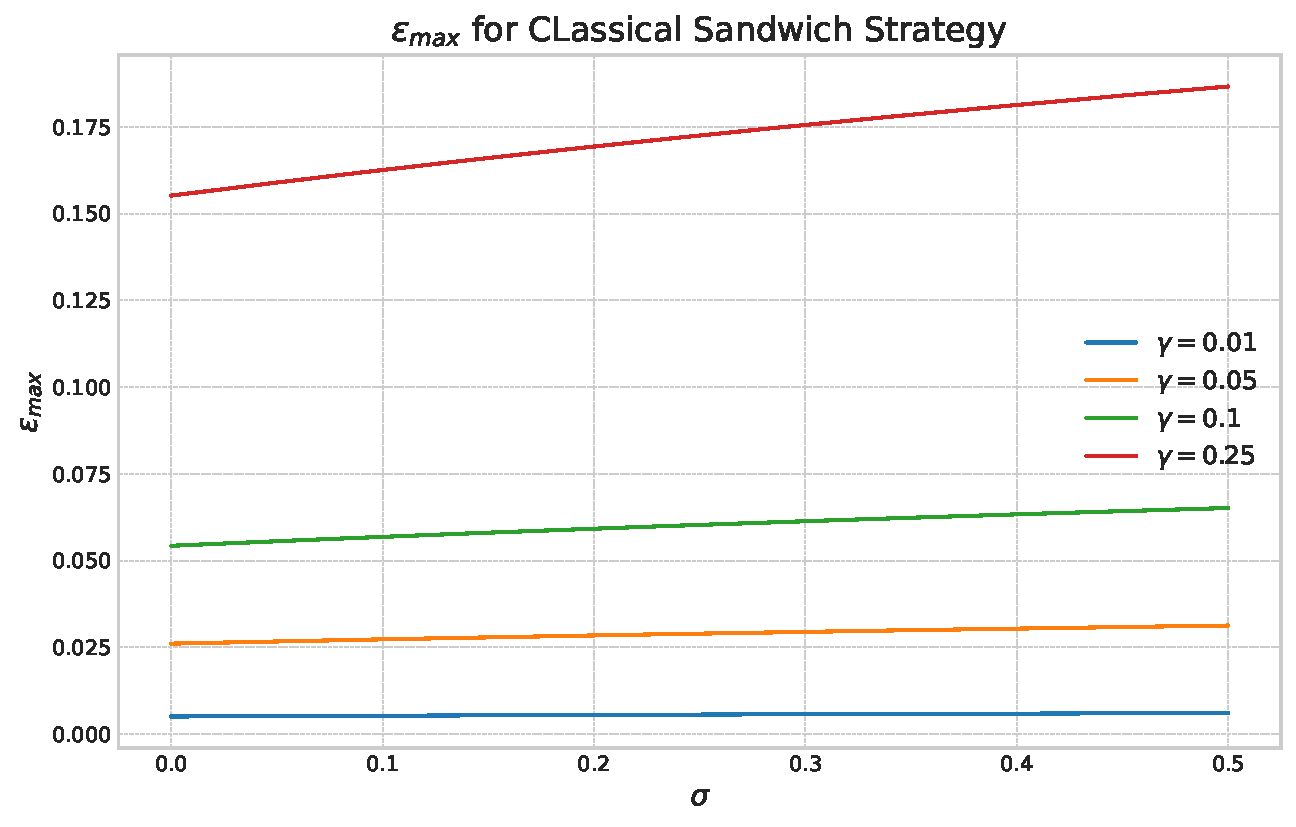
\includegraphics[width=0.7\linewidth]{figures_st_app/epsilon_max_sand.pdf}
    \caption{Caption}
    \label{fig:eps_max}
\end{figure}

%---------------------------------------------------------------------------
\paragraph{Back-run swap (Y$\to$X).} Finally, $\Delta y_{\mathrm{fr}}$ are traded back in the back-run swap from $Y$ to $X$. The amount that the searcher gets back is

\begin{equation}
\Delta x_{\text{br}} = x_0\frac{r^2 \varepsilon (1 + r\varepsilon + r\sigma)^2}{(1 + r\varepsilon) + r^2 \varepsilon (1 + r\varepsilon + r\sigma)}.
\end{equation}


%---------------------------------------------------------------------------
Not considering for the moment gas and bribe costs, the searcher's profit is the difference between the input amount in the front-run swap and the output amount in the back-run swap

\begin{equation}
\Pi_{sand}(\varepsilon, \sigma) = \Delta x_{\text{br}} - s = x_0 \left[\frac{r^2 \varepsilon(1 + r\varepsilon + r\sigma)^2}{(1 + r\varepsilon) + r^2 \varepsilon (1 + r\varepsilon + r\sigma)} - \varepsilon \right]
,
\label{eq:Pi_exact}
\end{equation}

\begin{equation}
\pi_{sand}(\varepsilon, \sigma) = \frac{\Pi}{x_0}
\label{eq:pi_exact}
\end{equation}

We can obtain the value of $\sigma$ that turn on the profits:

\begin{equation}
    \pi_{sand}(\varepsilon, \sigma) >0 \quad \text{when} \quad \sigma>\sigma_{min} = \frac{1}{r}\left(\frac{\varepsilon+\sqrt{\varepsilon^2 + \frac{4(1+r\varepsilon)}{r^2}}}{2}-1 - r\varepsilon \right) \underset{\varepsilon\to0^+}\approx f
\end{equation}
%---------------------------------------------------------------------------
Now we want to obtain the optimal value to trade in the front-run swap that maximizes the profit. In other words, we want to solve the following problem
\begin{align}
    \text{maximize } & \  \pi_{sand}(\varepsilon, \sigma) \nonumber\\ 
    \text{subject to } & \varepsilon \leq \varepsilon_{\text{max}}(\sigma, \gamma, r)
\end{align}
The first-order condition leads to a quartic equation whose solution can be found numerically. 

The constraint given by the slippage requires that the actual maximum $\varepsilon^*$ be
\begin{equation}
    \varepsilon^* = \min{\{\varepsilon_+, \varepsilon_{\text{max}}(\sigma, \gamma, r)\}}
\end{equation}
If we substitute this value in the profit expression, we get
\begin{equation}
    \pi_{sand}^*(\varepsilon,\sigma) = \frac{r^2 \varepsilon^* (1 + r\varepsilon^* + r\sigma)^2}{(1 + r\varepsilon^*) + r^2 \varepsilon^* (1 + r\varepsilon^* + r\sigma)} - \varepsilon^*
\end{equation}

%---------------------------------------------------------------------------
%  3.3  Sandwich attack option — size-based dominance
%---------------------------------------------------------------------------

Define the gas spread and the gas spread per reserve.
\begin{equation}
\delta' := G_{\text{JIT}}-G_{\text{sand}},\qquad
\phi'   := \frac{\delta'}{x_{0}}\quad
\end{equation}
The two bribe ceilings are

\[
\begin{aligned}
m_{\max}^{\text{JIT}} 
   &= S f - G_{\text{JIT}}
   = x_0\sigma f - G_{\text{JIT}}, \\
m_{\max}^{\text{sand}} 
   &= x_0 \pi^* - G_{\text{sand}}.
\end{aligned}
\]
and therefore
\[
m_{\max}^{\text{JIT}} \ge m_{\max}^{\text{sand}}
\quad\Longleftrightarrow\quad
\sigma f - \pi^* - \phi' \ge 0,
\qquad
\phi'=\frac{G_{\text{JIT}}-G_{\text{sand}}}{x_0}.
\]

The builder includes the JIT bundle when its
bribe ceiling exceeds the sandwich one:

\begin{equation}
x_{0}\,\bigl(\sigma f - \phi'\bigr)
   \;\ge\;
x_{0}\,\pi^*
\quad\Longleftrightarrow\quad
F(\sigma)\;:=\;
\sigma f - \phi' - \pi^*\;\ge 0.
\end{equation}

Because \(F(0)=-\phi' < 0\) (if JIT has any gas handicap)
and \(F(\sigma)\to \infty\) as \(\sigma\to\infty\),
there is (under regular fee-tier ranges) a unique positive root
\(\sigma_{\text{sand}}^{\ast}\) that solves \(F(\sigma)=0\). Therefore, we have that the JIT strategy wins against the sandwich attack alternative when

\begin{equation}
\boxed{%
   \sigma \;\ge\; \sigma_{\text{sand}}^{\ast}(f,\phi')
}
\qquad\Longleftrightarrow\qquad
\boxed{%
   S      \;\ge\; S_{\text{sand}}^{\ast}:=
            \sigma_{\text{sand}}^{\ast}\,x_{0}
}.
\end{equation}

Figure \ref{fig:frontrun_size_vs_profit} represents the relationship between the front-run size $\varepsilon$ and the sandwich profit $\pi(\varepsilon)$. As we can see, the profit reaches a maximum and then starts to decreases afterward. The decreasing can also lead to negative profits, especially for low liquidity pools. However, the maximum is never actually reached by the searcher. Also in this case, the slippage tolerance does not let the attacker to extract the most of the rent.

\subsection{Mixed (Sandwich + JIT) attack}
\label{subsec:mixed-sandwich-jit}

We analyze a bundle that combines a self-funded sandwich with JIT liquidity provision. The sequence consists of a front-run swap, a front-run mint, a set of victim swaps, a back-run burn, and a back-run swap. The goal is to profit both from the sandwich’s price impact and the JIT fee capture. Because the JIT deepens the book during the victim leg, the victim’s min-out constraint is easier to satisfy, which allows a larger feasible front-run size~$\varepsilon$. To the best of out knowledge, there is currently no study in the literature that accounts for this strategy. Furthermore, we were not able to find any particular information even on the web, even if data clearly shows the occurrence of this pattern, as highlighted in \cite{gatta_di_nosse}

\paragraph{Front-run swap (X$\to$Y).}
The attacker swaps $s=\varepsilon x_0$ (user input), so the effective input is $r s$. With constant product and fee on input,
\begin{equation}
  \Delta y_{\mathrm{fr}} \;=\; y_0\,\frac{r\varepsilon}{1+r\varepsilon},
  \qquad
  (x_0,y_0)\mapsto (x_1,y_1)=\bigl(x_0(1+r\varepsilon),\, y_0/(1+r\varepsilon)\bigr).
  \label{eq:mix_dyfr}
\end{equation}

\paragraph{Front-run JIT mint.}
To avoid changing price, it is convenient to parametrize the added reserves with respect to the current ones. If $\alpha$ of the \emph{post-FR} reserves is added, the state scales as
\begin{equation}
  (x_1,y_1) \;\mapsto\; (x_2,y_2) \;=\; \bigl(x_1(1+\alpha),\, y_1(1+\alpha)\bigr)
  \;=\; \Bigl(x_0(1+r\varepsilon)(1+\alpha),\, \frac{y_0(1+\alpha)}{1+r\varepsilon}\Bigr).
  \label{eq:mix_mint}
\end{equation}
Therefore the attacker owns a a fraction $\frac{\alpha}{\alpha + 1}$ of the active range.

\paragraph{Victim swap(s) (X$\to$Y).}
Size $S=\sigma x_0$; effective input $rS$. From \eqref{eq:mix_mint}, the victim’s Y out is
\begin{equation}
  \Delta y_v
  \;=\; \left(\frac{y_0}{1+r\varepsilon}\right)\!\cdot
         \frac{(1+\alpha)\,r\sigma}{(1+r\varepsilon)(1+\alpha)+r\sigma},
  \label{eq:mix_dyv}
\end{equation}
and the state becomes (still with JIT present)
\begin{equation}
  (x_3,y_3) \;=\;
  \Bigl(x_0\bigl((1+r\varepsilon)(1+\alpha)+r\sigma\bigr),\;
        \frac{y_0(1+\alpha)^2}{(1+r\varepsilon)(1+\alpha)+r\sigma}\Bigr).
  \label{eq:mix_state_with_jit_after_victim}
\end{equation}
Slippage feasibility is the same as in §3.3 but in this case the enhanced liquidity allows for a bigger $\varepsilon_{\text{max}}$ (see Figure \ref{fig:eps_max_jit_sand}):
\begin{equation}
  \Delta y_v \;\ge\; (1-\gamma)\,\Delta y_{\mathrm{base}},
  \quad \Delta y_{\mathrm{base}}=y_0\,\frac{r\sigma}{1+r\sigma},
  \quad\Longrightarrow\quad
  \varepsilon \le \varepsilon_{\max}(\sigma,\gamma,r, \alpha).
  \label{eq:mix_eps_cap}
\end{equation}
where

\begin{equation}
    \varepsilon_{\max}(\sigma,\gamma,r, \alpha) = \frac{1}{r}\left[\frac{-r\sigma + \sqrt{(r\sigma)^2+ \frac{4(1+\alpha)^2(1+r\sigma)}{1-\gamma}}}{2(1+\alpha)}-1 \right]
\end{equation}

\begin{figure}
    \centering
    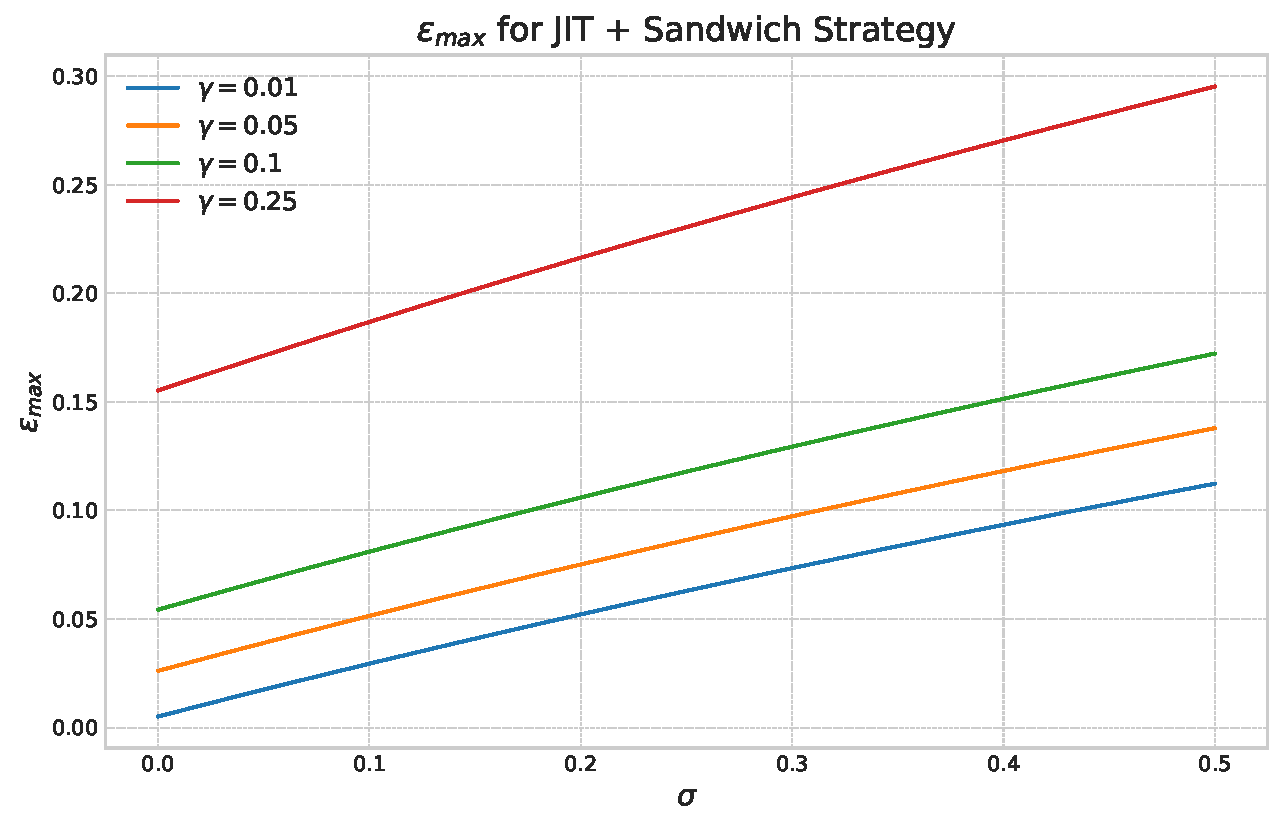
\includegraphics[width=0.7\linewidth]{figures_st_app/epsilon_max_jit_sand.pdf}
    \caption{Maximum normalized front run amount $\epsilon_{max}$ vs normalized victim's swap amount $\sigma$ for different values of the slippage tolerance $\gamma$. The value of $\alpha$ is set to 1 (i.e. LP owns half of the active tick range).}
    \label{fig:eps_max_jit_sand}
\end{figure}

\paragraph{Back-run burn (JIT).}
Immediately after the victim, the JIT LP is burned. Since the position was proportional, burning removes a fraction $\alpha/(1+\alpha)$ of both reserves, so the base-pool state is
\begin{equation}
  (x_4,y_4) \;=\; \frac{1}{1+\alpha}\,(x_3,y_3)
 \;=\; \Bigl(x_0\bigl((1+r\varepsilon)+\frac{r\sigma}{1+\alpha}\bigr),\;
             \frac{y_0(1+\alpha)}{(1+r\varepsilon)(1+\alpha)+r\sigma}\Bigr).
  \label{eq:mix_state_after_burn}
\end{equation}
After the burn, the attacker ends up with 
\begin{equation}
    \Delta x_{\mathrm{burn}}
    = \frac{\alpha}{1+\alpha}\,x_3
    = \alpha x_0(1+r\varepsilon) + \frac{\alpha}{1+\alpha}\,r\sigma x_0.
\end{equation}
$\alpha x_0(1+r\varepsilon) + \frac{\alpha}{1+\alpha}r \sigma x_0$ tokens $X$ and $\frac{\alpha y_0}{1+r\varepsilon} - \frac{\alpha}{1+\alpha}\Delta y_v$ tokens $Y$.

\paragraph{Back-run swap (Y$\to$X).}
The attacker now has to swap in the opposite direction than victims' swaps. 

\begin{equation}
    x_4 y_4 = \bigl( x_4 - \Delta x_{br}\bigr)\bigl(y_4 + r\Delta y_{br}\bigr)
\end{equation}

We can derive the expression of $\Delta x_{br}$ with respect to $x_0$. Let $\theta = \frac{\Delta y_{br}}{y_0}$

\begin{equation}
\Delta x_{br} = x_0 \left\{\frac{\left[(1+r\varepsilon)(1+\alpha) + r\sigma\right]^2r\theta}{(1+\alpha)\left[(1+\alpha) + \left((1+\alpha)(1+r\varepsilon)+r\sigma\right)r\theta\right]} \right\}
\end{equation}

\paragraph{Profit.} The profit the attacker obtains is composed of the difference between the back-run output amount and the front-run input amount (the same as in the case of the classical sandwich) plus the fees collected by the LP position plus the difference between the tokens' amounts burnt and minted

\begin{equation}
    \Pi_{sand+jit}(\varepsilon,\sigma, \alpha) = \underbrace{\bigl(\Delta x_{br} - \varepsilon x_0 \bigr)}_{\text{Sandwich}} + \underbrace{\sigma x_0f\frac{\alpha}{\alpha + 1}}_{\text{LP fees}} + \underbrace{x_0\alpha r \sigma \left[\frac{1}{1+\alpha}-\frac{1}{(1+r\varepsilon) \left( (1+\alpha)(1+r\varepsilon)+r\sigma\right)}\right]}_{\text{LP inventory}}
\end{equation}

Therefore, normalizing the profit with respect to $x_0$ and substituting the full expression for $\Delta x_{br}$, we obtain
\begin{equation}
\begin{aligned}
\pi_{sand+jit}(\varepsilon, \alpha, \sigma) 
= &\left\{ \frac{\left[(1+r\varepsilon)(1+\alpha) + r\sigma\right]^2 r\theta}
{(1+\alpha)\left[(1+\alpha) + \left((1+\alpha)(1+r\varepsilon)+r\sigma\right)r\theta\right]} - \varepsilon \right\} \\
&+ \frac{\sigma f \alpha}{\alpha + 1} 
+ \alpha r \sigma \left[ \frac{1}{1+\alpha} - \frac{1}{(1+r\varepsilon)\left((1+\alpha)(1+r\varepsilon)+r\sigma\right)} \right]
\end{aligned}
\end{equation}


In general, we have two options for $\theta y_0$
: (i) keep the self funding framework as in the classical sandwich attack or (ii) let the back run amount to be a new free parameter. Currently we did not study the second option since empirically we almost always find the self funded option, as we can see from Figure \ref{fig:obs_vs_pred_backrun}.

\begin{figure}
    \centering
    
\includegraphics[width=0.5\linewidth]{figures_st_app/obs_vs_pred_backrun.pdf}
    \caption{Relation between the back run swap amount observed on-chain $\Delta y_{br}^{obs}$ and the theoretical one $\Delta y_{br}$ based on the self funding condition.}
    \label{fig:obs_vs_pred_backrun}
\end{figure}

Differently from the case of the self funded sandwich attack, in this case the back run amount is not equal to the front run amount, because the LP position has already hedged part of the attacker exposure obtained after the front run. Specifically, during the victims' swap, the attacker takes the opposite side of the trades, giving $\frac{\alpha}{ (1+\alpha)}\Delta y_v$ tokens $Y$ and receiving $\frac{\alpha}{ (1+\alpha)}rS$ of tokens X. Therefore, she has only to back run the residual $\theta_{self} = \frac{1}{y_0}\left(\Delta y_{fr} - \frac{\alpha}{1+\alpha} \Delta y_v\right)$. Empirically it is actually what we see.

In this case, the LP inventory change in tokens Y is fed as a minus component into the back run amount. The profit is therefore 

\begin{equation}
    \Pi_{\mathrm{sand+jit}}(\varepsilon, \alpha, \sigma)
    = \Delta x_{\mathrm{br}}(\theta_{\mathrm{self}}) - \varepsilon x_0 + \frac{\alpha}{1+\alpha}\,\sigma x_0
\end{equation}

The full expression is

\begin{equation}
\pi_{sand+jit}(\varepsilon, \alpha, \sigma) = \frac{[(1 + r\varepsilon)(1 + \alpha) + r\sigma ]^2r\theta_{self}}{(1 + \alpha)\left[(1 + \alpha) + ((1 + \alpha)(1 + r\varepsilon) + r\sigma) r\theta_{self}\right]} - \varepsilon + \frac{\alpha\sigma}{\alpha + 1}
\end{equation}

where
\begin{equation}
    \theta_{self} = \frac{r}{1+r\varepsilon} \left[\varepsilon - \frac{\alpha \sigma}{(1+r\varepsilon)(1+\alpha)+r\sigma}\right]
\end{equation}

When $\theta_{self}\leq0$ the (normalized) fees earned by the LP is bigger that $\epsilon$, flipping the sign of the back run swap. Therefore, to not incur in a loss, the MEV searcher chooses to perform a pure JIT.

The maximization problem is 

\begin{equation}
\begin{aligned}
\max_{\varepsilon,\alpha} \;\; \pi_{\text{sand+jit}} \quad \text{subject to} \quad
\begin{cases}
0 \leq \varepsilon \leq \varepsilon_{\max} \\
\alpha \geq 0 \\
\theta_{self} >0
\end{cases}
\end{aligned}
\end{equation}

The results have been obtained numerically searching for $\varepsilon^* \in [\varepsilon_{min}, \infty]$ and $\alpha \in [0, \alpha_{max}]$ with $\varepsilon_{min}=10^{-9}$ and $\alpha_{max} = 1$. Actually, the optimizer always pushes $\alpha^* \to \alpha_{max}$, whatever its value is. Figure \ref{fig:regime_transition} shows  $\varepsilon^*$ and $\alpha^*$ as a function of the normalized victim's input size $\sigma$ for $f=0.01\%, 0.05\%, 0.3\%$. Except in the case of the $0.01\%$, we can see that there is a quite sharp transition between two different regimes:

\begin{enumerate}
    \item Pure JIT, where $\varepsilon$ is pushed to $\varepsilon_{min}$ and $\alpha$ to $\alpha_{max}$
    \item Combination of JIT and Sandwich attack with 
\end{enumerate}

\begin{figure}
    \centering
    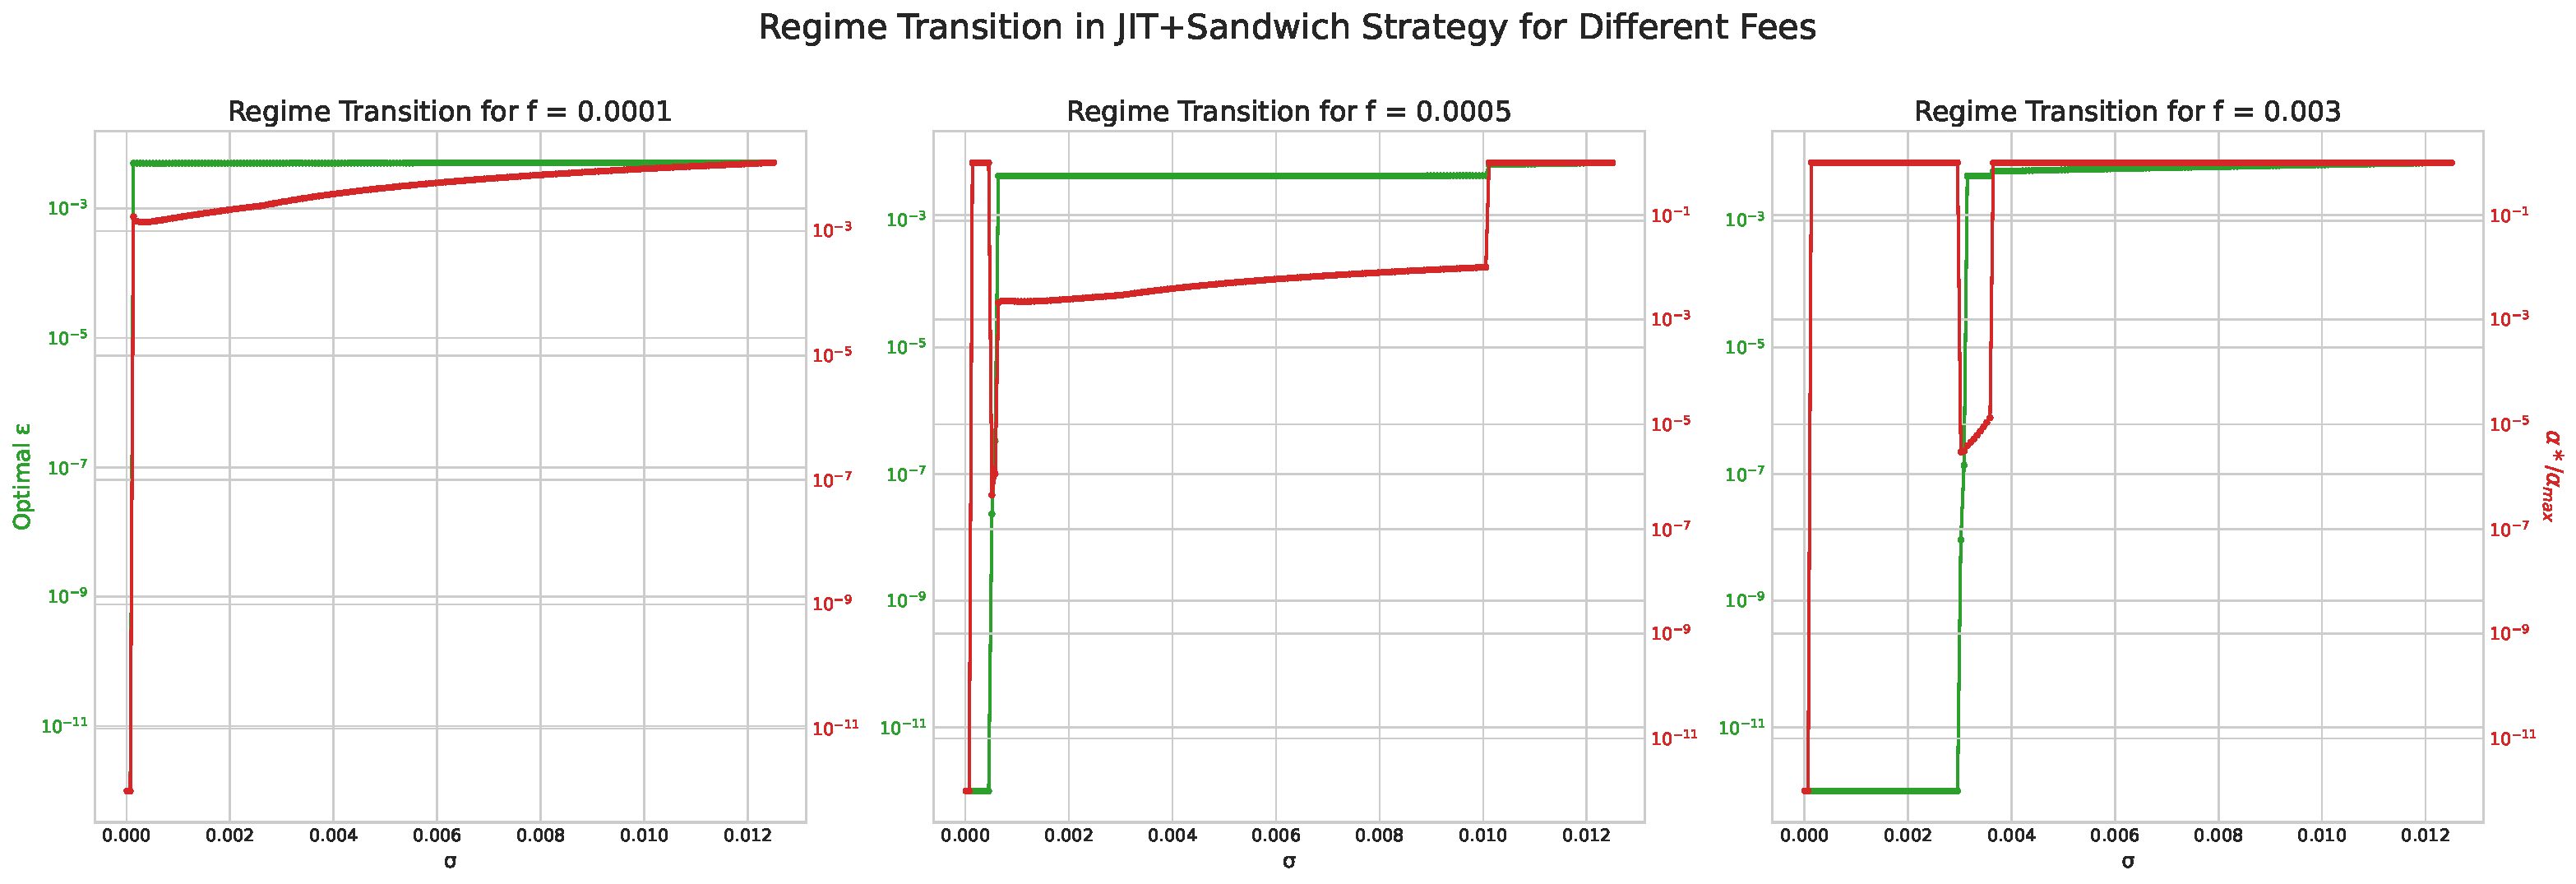
\includegraphics[width=1\linewidth]{figures_st_app/regime_transition_subplots.pdf}   \caption{Optimal values for $\varepsilon$ and $\alpha$ with respect to $\sigma$ for different values of the fee tier.}
    \label{fig:regime_transition}
\end{figure}

Figure \ref{fig:profits_comparison} shows the dynamics of the four ceilings (profits) for the three MEV strategies discussed so far for different fee tiers. One can be surprised by the fact that a classic sandwich attack is less profitable than an arbitrage trade after a certain value of $\sigma$. This is due to how we treated the sandwich attack strategy. Indeed, we set up a self funded strategy, in which the back run amount is equal to the front run size. Due to the presence of the slippage tolerance, the maximum front-run size $\varepsilon_{max}$ is limited. Therefore, also the maximum profit achievable will be affected by this constraint. On the other hand, we do not have any limit on the arbitrage back-run that depends only on the victim swapped size $\sigma$. Anyway, combining a classical sandwich with a JIT, allows for a greater front run size and a flow of fee towards the searcher. This makes the mixed strategy the most profitable one for $f=0.3\%$. For lower ones, the difference between the classical sandwich and the mixed strategy becomes negligible. As we can see from the graphs, the transition between a pure JIT and a mixed strategy happens at $\sigma=f$.


\begin{figure}
    \centering
     
\includegraphics[width=0.9\linewidth]{figures_st_app/profits_comparison.pdf}
    \label{fig:profits_comparison}
    \caption{Visualization of the profits of the different MEV strategies for $f\in[0.01\%,0.05\%,0.3\%]$ and slippage $\gamma=1\%$. The vertical gray dashed line corresponds to the minimum value of $\sigma$ that induces a price change greater than the fee tier, while the red dashed line highlights the pool's fee rate. The gas fees are set to zero.}
\end{figure}

\begin{figure}
    \centering
    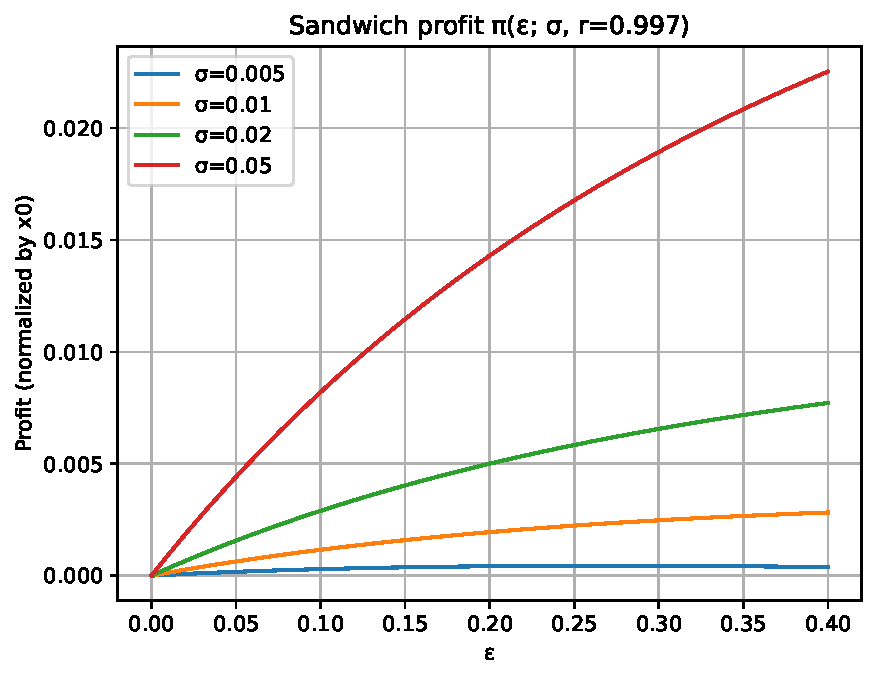
\includegraphics[width=0.7\linewidth]{figures_st_app/sandwich_profit_vs_epsilon.pdf}
    \caption{Sandwich profits vs $\varepsilon$. The vertical dashed lines correspond to th e maximum value of the front run size $\varepsilon_{max}(\gamma)$ for different value of the slippage tolerance $\gamma$. Fee tier 0.05\%, $x_0=1$.}
    \label{fig:frontrun_size_vs_profit}
\end{figure}

\section{Empirical profits}
Currently I have collected MEV patterns discussed in the previous sections for the 2023 and for the USDC-WETH 0.05\% pool. The goal is to check the validity of the relationship obtained in the previous section regarding the MEV strategy profits.

The heuristic used to collect the arbitrage swaps is inherently noisy: a swap that changed the price for a quantity greater than the fee tier is not necessarily followed by an arbitrage swap. In other words, even if there is a swap in the opposite direction, it can be a coincidence. Therefore, I applied a stronger heuristic, collecting only the swaps that pushed the price back to $1\%$ of the target $rP_0$.

Profits are evaluated based on actual on-chain data as the difference between what the searcher paid and what was obtained from the strategy. There is therefore no bias due to the theory discussed above, except for the condition imposed while collecting back run arbitrages.

Finally, no gas costs have been considered.

The JIT and classical sandwich attacks profits seem to follow the behavior obtained in the theoretical sections. However, for sandwich profits we found
\begin{itemize}
    \item A lot of negative profits. Almost all of them are related to $\sigma < \sigma_{min}$
    \item A lot of back run arbitrages with almost zero profits
\end{itemize}

As shown in Figure \ref{fig:empirical_profits} , there are some discrepancies between theory and empirical evidences. For instance, the onset of positive profits for both the sandwich attacks/mixed strategy and the back run arbitrages happens for $\sigma$ values a bit greater than the predicted ones. Possible sources of this discrepancy can be (i) not optimality in strategy settings or, more probably, (ii) cross-tick effects that we did not account for

\begin{figure}
    \centering
    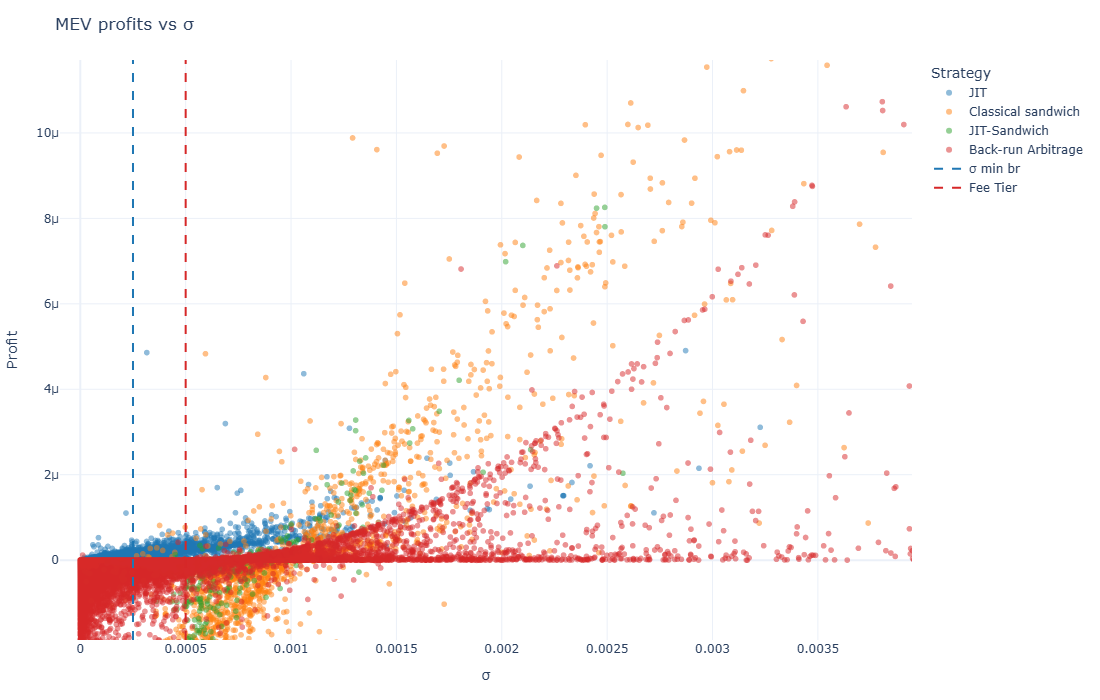
\includegraphics[width=0.7\linewidth]{figures_st_app/empirical_profits.png}
    \caption{Caption}
    \label{fig:empirical_profits}
\end{figure}

\appendix
\section{Tick-aware rules for Uniswap v3 execution}
\label{app:tick-rules}

\paragraph{State and notation.}
Let \(S=\sqrt{P}\) denote the square-root price (X in Y) and \(L\) the \emph{active} liquidity of the current tick whose boundaries are \((S_\ell,S_u)\) with \(S_\ell<S<S_u\).
The pool charges a fee-on-input \(f\); write \(r=1-f\).
For intuition within a tick, define the virtual reserves \(\tilde x=L/S\) and \(\tilde y=L\,S\) (so \(\tilde x\,\tilde y=L^2\)).
Only \emph{swaps} move price; \emph{mints/burns} are price-neutral.

\subsection{Swaps within a tick (price update and amounts)}
\label{app:swaps-within-tick}
\textbf{X\(\to\)Y (consume X, output Y).}
For effective input \(x_{\mathrm{eff}}=r\,x_{\mathrm{in}}\):
\begin{equation}
S'=\frac{1}{\,S^{-1}+x_{\mathrm{eff}}/L\,},\qquad
\Delta y = L\,(S'-S),\qquad
\text{fees in X} = f\,x_{\mathrm{in}}.
\end{equation}

\noindent
\textbf{Y\(\to\)X (consume Y, output X).}
For effective input \(y_{\mathrm{eff}}=r\,y_{\mathrm{in}}\):
\begin{equation}
S' = S + \frac{y_{\mathrm{eff}}}{L},\qquad
\Delta x = L\Big(S^{-1}-S'^{-1}\Big),\qquad
\text{fees in Y} = f\,y_{\mathrm{in}}.
\end{equation}

\noindent\emph{Interpretation.}
Within a tick these are exactly the constant-product updates on \((\tilde x,\tilde y)\) using the \emph{effective} input \(r\) (fees are withheld from input and added to the pool in the input token).
Signs \(\Delta x,\Delta y\) above are pool-side deltas (amounts received by the trader have opposite sign).

\subsection{Tick boundaries (capacity and traversal)}
\label{app:boundaries}
\textbf{Capacity to the lower boundary} \(S_\ell\) for a \emph{downward} move (X\(\to\)Y):
\begin{equation}
x_{\max}^{(\mathrm{eff})}=L\!\left(\frac{1}{S_\ell}-\frac{1}{S}\right),\qquad
x_{\max}= \frac{x_{\max}^{(\mathrm{eff})}}{r}.
\end{equation}

\noindent
\textbf{Capacity to the upper boundary} \(S_u\) for an \emph{upward} move (Y\(\to\)X):
\begin{equation}
y_{\max}^{(\mathrm{eff})}=L\,(S_u-S),\qquad
y_{\max}=\frac{y_{\max}^{(\mathrm{eff})}}{r}.
\end{equation}

\noindent
\textbf{Boundary rule.}
When a boundary is reached, update the active liquidity
\begin{equation}
L \leftarrow L \pm \Delta L_{\mathrm{tick}},
\end{equation}
where \(\Delta L_{\mathrm{tick}}\) is the net liquidity change encoded at that boundary; then advance to the next active tick \((S_\ell,S_u)\) and continue.
(Only the \emph{active} tick’s \(L\) affects price moves.)

\subsection{Liquidity changes (mints and burns)}
\label{app:mints-burns}
\paragraph{General mint (range \([\;S_a,S_b\;]\) with \(S_a<S_b\)).}
Adding \(\Delta L\) does \emph{not} move price.
The deposited principal amounts at current \(S\) are
\begin{equation}
(\Delta x,\Delta y)=
\begin{cases}
\Big(\Delta L\!\big(\dfrac{1}{S_a}-\dfrac{1}{S_b}\big),\; 0\Big), & S\le S_a,\\[8pt]
\Big(\Delta L\!\big(\dfrac{1}{S}-\dfrac{1}{S_b}\big),\; \Delta L\,(S-S_a)\Big), & S_a<S<S_b,\\[8pt]
\Big(0,\; \Delta L\,(S_b-S_a)\Big), & S\ge S_b.
\end{cases}
\end{equation}
If \(S\in[S_a,S_b)\), the position is \emph{active} and the active liquidity becomes \(L\leftarrow L+\Delta L\).
If \(S\notin[S_a,S_b)\), the deposit is \emph{inactive now} (no change to active \(L\)) and becomes active only when price re-enters the range.

\paragraph{JIT mint (ultra-narrow around the current tick).}
Take \([S_a,S_b]\) to coincide with the current tick; set \(\alpha=\Delta L/L_{\mathrm{base}}\).
Then, while price stays in the tick,
\begin{equation}
L \leftarrow (1+\alpha)\,L_{\mathrm{base}},\qquad
(\tilde x,\tilde y)\ \text{scale by }(1+\alpha).
\end{equation}
This is the formal justification for the “state scales by \(1+\alpha\)” step used in Section~3.
If price leaves the tick before a burn, the JIT position becomes \emph{inactive} (it no longer contributes to active \(L\)) until price re-enters or the position is burned.

\paragraph{General burn (range \([\;S_a,S_b\;]\)).}
Removing \(\Delta L\) does \emph{not} move price.
The withdrawn principal at current \(S\) is
\begin{equation}
(\Delta x,\Delta y)=
\begin{cases}
\Big(\Delta L\!\big(\dfrac{1}{S_a}-\dfrac{1}{S_b}\big),\; 0\Big), & S\le S_a,\\[8pt]
\Big(\Delta L\!\big(\dfrac{1}{S}-\dfrac{1}{S_b}\big),\; \Delta L\,(S-S_a)\Big), & S_a<S<S_b,\\[8pt]
\Big(0,\; \Delta L\,(S_b-S_a)\Big), & S\ge S_b.
\end{cases}
\end{equation}
If the position is \emph{active} at burn time, update active liquidity \(L\leftarrow L-\Delta L\).
If the position is \emph{inactive}, burning does not change active \(L\) (you still withdraw principal computed at current \(S\) per the cases above).

\paragraph{Fee accruals for mints/burns.}
Fees are collected \emph{pro-rata to active liquidity and only while the position is active}.
In a swap that consumes input \(q\) with fee \(f\), the pool retains \(f\,q\) of the \emph{input} token; a position active during that swap accrues the share
\(\dfrac{\Delta L}{L_{\mathrm{active}}}\times f\,q\)
(up to rounding) into its uncollected fees.
Burning (or an explicit \texttt{collect}) realizes the position’s uncollected fees in their respective tokens \emph{in addition to} the principal amounts above.
For a JIT mint active only for the victim swap, the fee share during that swap is \(\dfrac{\alpha}{1+\alpha}\) of the victim’s fee in the input token (again subject to rounding and any protocol fee).


% \section{Empirical Analysis of MEV on Uniswap v3}
% In this section we provide an empirical analysis on the frequency and characteristic of some of the MEV strategies discussed in the previous section. Specifically, we focus on collecting, using the public available onchain data, arbitrage, sandwich attack and JIT liquidity events. Then, we evaluate the profitability of these strategies.

% The study period covers the entire 2023 and 2024. Specifically, we focus on the 24 most active pools\footnote{By "most active" we mean "with the biggest number of events" (swaps+mints+burns). Specifically, we consider pools with at least 40,000 events recorded in the study period.}, which involve 15 token pairs. The data are retrieved using the official Ethereum subgraph of Uniswap v3 hosted by TheGraph \footnote{Further details can be found on the webpage \url{https://https://github.com/tradingstrategy-ai/web3-ethereum-defi} and \url{https://thegraph.com/explorer/subgraphs/5zvR82QoaXYFyDEKLZ9t6v9adgnptxYpKpSbxtgVENFV?view=Query&chain=arbitrum-one}, respectively.}. Both methods provide standardized and reliable access to on-chain DeFi information.


% \subsection{Just-in-Time Liquidity}
% Liquidity provision has traditionally been viewed as a passive activity, where liquidity providers (LPs) deposit tokens into pools and await liquidity takers (LTs) to execute trades. In contrast, Just-in-Time (JIT) liquidity, as introduced by Wan et al. (2022) and further discussed by Capponi et al. (2023), represents a form of active liquidity management. The primary objective of JIT liquidity is to minimize the periods when LP tokens remain unused, thereby reducing exposure to adverse selection. Specifically, upon identifying a significant swap transaction in the Ethereum mempool, an MEV searcher can promptly provide liquidity tailored to that swap. Consequently, the searcher's liquidity is utilized and withdrawn within the same blockchain block, allowing them to collect trading fees without long-term exposure.

% The JIT liquidity provision typically exhibits a distinctive transactional pattern within a single block: an initial mint transaction with an extremely narrow tick range (often the narrowest possible range defined by the protocol's tick spacing), followed by the targeted victim swap transaction(s), and concluding with a burn transaction that removes precisely the previously minted liquidity. Our detection algorithm exploits this identifiable sequence. Specifically, we analyze each pool individually, scanning mint events for occurrences paired with a corresponding burn transaction executed by the same wallet within the same block, completely withdrawing the minted liquidity. Crucially, we require at least one swap transaction to occur between the mint and burn events. Unlike prior methodologies that demand the three events (mint, swap, burn) be strictly consecutive within a block, our approach relaxes this constraint. We only enforce that the log indices of these events follow the order mint < swap < burn, thus including instances where intervening transactions occur. This adjustment acknowledges that intervening transactions do not affect the economic incentives or profitability underlying JIT liquidity strategies.

% JIT liquidity attacks generally yield advantageous outcomes for liquidity takers (LTs), as they substantially mitigate the swap's price impact by injecting additional liquidity into the pool. Although referring to the primary swap in a JIT scenario as a "victim" may slightly misrepresent the beneficial nature for the LT, we retain this terminology for consistency with existing MEV and sandwich attack literature. Additionally, executing a JIT attack results in the attacker acquiring a positive exposure to the asset sold by the LT and a negative exposure to the asset bought by the LT. Given that the attacker essentially serves as the main counterparty for the LT during the swap, they typically manage this risk by hedging their positions through trades on alternative decentralized or centralized exchanges (DEXs or CEXs), as noted by Wan et al. (2022).

% JIT liquidity attacks generally yield advantageous outcomes for liquidity takers (LTs), as they substantially mitigate the swap's price impact by injecting additional liquidity into the pool. Although referring to the primary swap in a JIT scenario as a "victim" may slightly misrepresent the beneficial nature for the LT, we retain this terminology for consistency with existing MEV and sandwich attack literature. Additionally, executing a JIT attack results in the attacker acquiring a positive exposure to the asset sold by the LT and a negative exposure to the asset bought by the LT. Given that the attacker essentially serves as the main counterparty for the LT during the swap, they typically manage this risk by hedging their positions through trades on alternative decentralized or centralized exchanges (DEXs or CEXs), as noted by Wan et al. (2022).

% To effectively capture nearly all the fees paid by the LT, the liquidity minted by active LPs during JIT attacks is typically substantially larger than that of passive LPs. For instance, Figure \ref{img:jit_liq_vs_nonjit_liq} illustrates the Kernel Density Estimation (KDE) comparison between liquidity minted by passive and active LPs in the USDC-WETH 0.05\% pool. The active LPs mint significantly more liquidity due to their very narrow tick range strategy.

% \begin{figure}[h]
% \centering
% 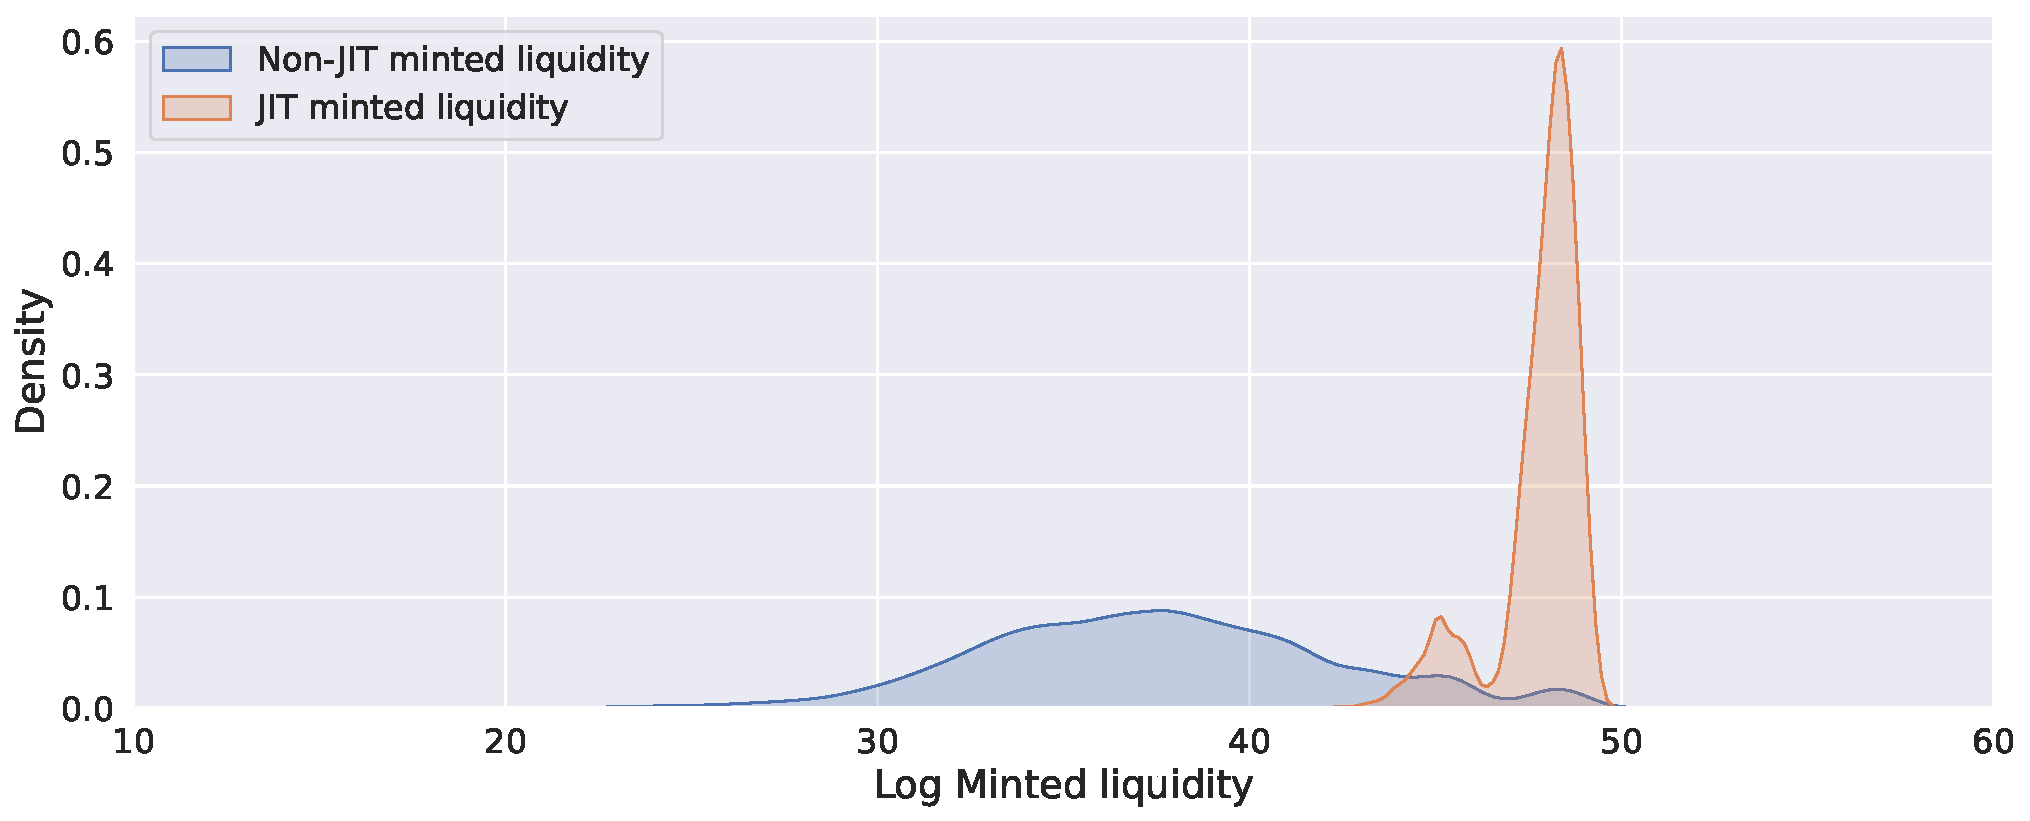
\includegraphics[scale=0.35]{figures_st_app/jit_vs_non_jit_minted_liquidity_kde_sns.pdf}
% \caption{Distribution comparison of log liquidity minted by JIT liquidity versus non-JIT liquidity providers in the USDC-WETH 0.05\% pool. JIT liquidity tends to cluster towards higher liquidity values, primarily due to the narrowly defined tick ranges used by attackers.}
% \label{img:jit_liq_vs_nonjit_liq}
% \end{figure}

% Figure \ref{fig:enter-jit_impact_x_paper} further explores the broader impact of JIT strategies on pool dynamics. It presents the proportion of mint events, the total liquidity minted, and the volume of victim swaps associated with JIT attacks.

% \begin{figure}
% \centering
% 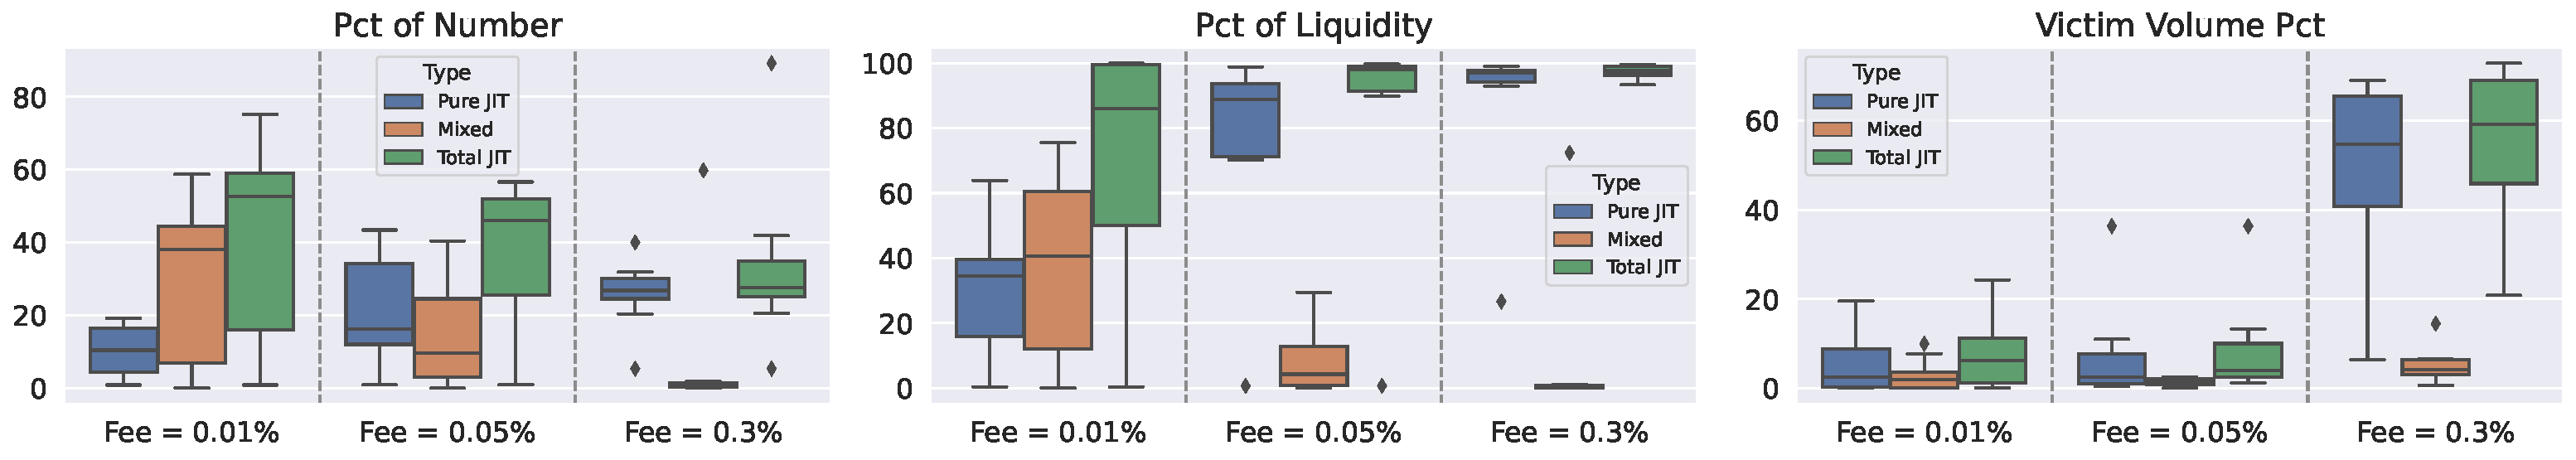
\includegraphics[height=0.17\linewidth]{figures_st_app/jit_impact_x_paper.pdf}
% \caption{Impact of JIT liquidity provision strategies: The left plot displays the percentage of mint events categorized as JIT; the center plot illustrates the percentage of minted liquidity from JIT activities; the right plot shows the proportion of total swap volume targeted by sandwich attacks. Each box differentiates pools based on fee tiers, with blue boxes indicating pure JIT attacks, orange boxes representing mixed JIT-sandwich attacks, and green boxes aggregating all JIT-related activities.}
% \label{fig:enter-jit_impact_x_paper}
% \end{figure}

% Summarizing our findings, JIT liquidity provisions constitute over 20\% of all mint operations and more than 50\% of minted liquidity within our dataset. Remarkably, this figure rises to approximately 90\% when focusing specifically on pools with 0.05\% and 0.3\% fee tiers, partly influenced by the characteristically narrow tick ranges in these JIT events. These findings underscore the concept of active liquidity provision as articulated by Capponi et al. (2023), emphasizing that JIT activities have become a significant component of market operations rather than isolated profit-seeking opportunities. Furthermore, clear distinctions emerge among fee tiers, with pure JIT attacks predominantly profitable in pools with higher fees.\\

% In line with previous work by Xiong et al. (2023), we further examine the composition of active liquidity providers. Their analysis revealed that more than 70\% of all JIT transactions were historically executed by a single user, though their data spanned from June 2021 to January 2023, overlapping with our dataset only in January 2023. Extending their analysis temporally, we investigate subsequent developments over the following two years. By collecting active LP wallet addresses, we quantify the transaction activity per wallet. We find a more distributed environment, though a single MEV bot, publicly recognized as "jaredfromsubway" (wallet address 0xae2Fc483527B8EF99EB5D9B44875F005ba1FaE13), still accounts for approximately 26\% of all JIT transactions. Additionally, 13 accounts individually constitute at least 2\% of transactions, with this number increasing to 25 and 42 accounts when thresholds are lowered to 1\% and 0.5\%, respectively. This indicates a gradual diversification in the pool of active JIT providers.

% Conversely, mixed attacks remain notably centralized, with the same "jaredfromsubway" bot responsible for around 88\% of these activities. Only three attackers surpass 1\% and 2\% thresholds, whereas five exceed the 0.5\% threshold, highlighting the concentrated nature of mixed attack operations.

% \subsection*{Example}
% A trader submits a Uniswap swap of 1{,}000 ETH for USDC. A Just-in-Time (JIT) LP detects this in the mempool and mints a concentrated liquidity position moments before the transaction.

% \begin{itemize}
%     \item Pool fee: 0.3\%
%     \item ETH price: \$3{,}300
%     \item Swap size: 1{,}000 ETH
%     \item Price impact on CEX (0.1\%): \$3{,}300
%     \item Exchange fee on CEX (0.05\%): \$1{,}650
%     \item Gas fees and tips: \$500
% \end{itemize}

% \begin{align}
% \text{Revenue (Fee earned)} &= 1{,}000 \times 0.003 = 3~\text{ETH}
% \Rightarrow 3 \times 3{,}300 &= \$9{,}900 \notag \\
% \text{Total Cost} &= 3{,}300 + 1{,}650 + 500 = \$5{,}450 \notag \\
% \text{Net Profit} &= \$9{,}900 - \$5{,}450 = \boxed{\$4{,}450} \notag
% \end{align}


% \subsection{Sandwich Attacks}
% \label{subsec:sand_att}
% Sandwich attacks occur when MEV searchers exploit large swaps pending in the mempool, aiming to profit from the resulting price impact. To execute such an attack, the searcher strategically places swaps immediately before and after the targeted victim’s swap. More explicitly, if we denote by $\epsilon$ the victim’s swap direction—either +1 if swapping from token X to token Y, or -1 otherwise—the general sandwich pattern consists of an attacker’s initial swap in direction $\epsilon$, followed by one or more victim swaps in the same direction, and concluded by the attacker’s final swap in direction $-\epsilon$. This strategy negatively impacts the victim by unfavorably shifting prices, causing the victim to buy at higher prices or sell at lower ones.

% To identify sandwich attacks, our algorithm examines each liquidity pool individually and scans blocks containing at least three swaps. We search for pairs of opposite-direction swaps executed by the same wallet within a block. If there is at least one intermediate swap by another wallet moving in the same direction as the attacker’s initial swap, we classify this sequence as a sandwich attack\footnote{In theory, an attacker could use multiple wallets—for instance, transferring tokens from the initial wallet to another before executing the back-run swap. While this incurs additional gas fees, the feasibility of such strategies remains uncertain and might partially explain discrepancies in sandwich counts across studies, as noted by \cite{li2024geth}. Further investigation into multi-wallet attacks remains an open area for research.}.

% Throughout the entire observation period, we identified 36,353 sandwich attacks targeting the USDC-WETH pair. Table \ref{tab:sandwich_attacks} provides a detailed breakdown, revealing that most attacks concentrate within pools featuring lower fee tiers.

% \begin{table}[h!]
% \centering
% \begin{tabular}{|l|r|r|r|}
% \hline
% \textbf{Pattern} & \textbf{0.01\%} & \textbf{0.05\%} & \textbf{0.30\%} \\ \hline
% Classical sandwich & 29054 & 3889 & 5 \\ \hline
% JIT sandwich & 1127 & 2271 & 7 \\ \hline
% \end{tabular}
% \caption{Counts of different sandwich attack types affecting the USDC-WETH pair, organized by pool fee tier.}
% \label{tab:sandwich_attacks}
% \end{table}

% The largest sandwich attack identified involved 11 intermediate swaps, although attacks featuring just a single victim swap represent approximately 95\% of all cases. Attacks involving two intermediate swaps account for around 4.5\%, while more complex patterns collectively represent less than 1\%. Figure \ref{img:sandwich} illustrates the Kernel Density Estimation (KDE) for the logarithm of the absolute USDC amounts swapped in sandwich attacks within the USDC-WETH 0.05\% pool.

% \begin{figure}[h]
% \centering
% 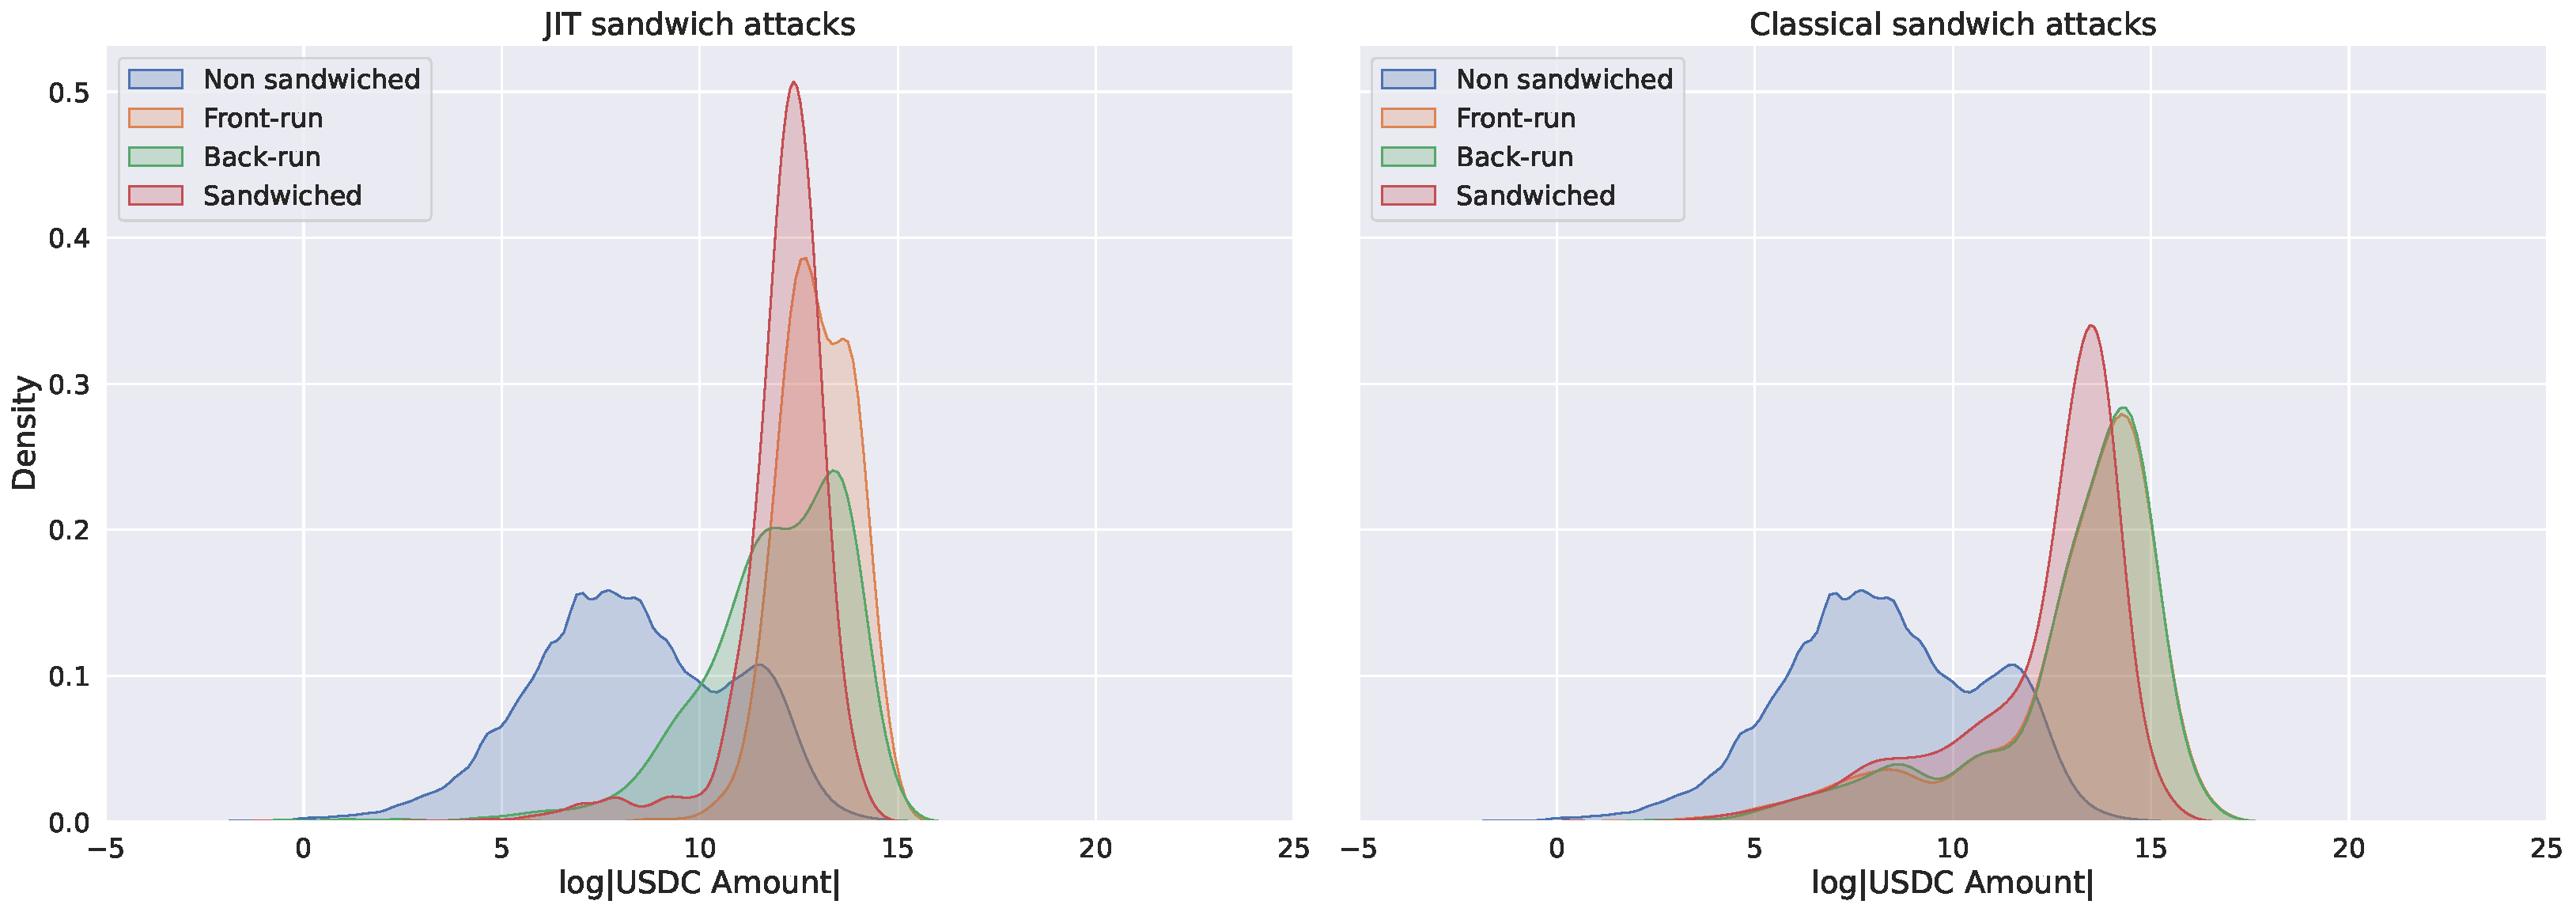
\includegraphics[width=1.0\textwidth]{figures_st_app/sandwiched_swaps_amounts_comparison.pdf}
% \caption{KDE distributions comparing the log of absolute USDC amounts swapped in sandwich attacks (36,353 cases) in the USDC-WETH 0.05\% pool. The left plot refers to mixed sandwich+JIT attacks, while the right plot focuses on pure sandwich attacks. Blue areas denote non-sandwich swaps, red areas represent victim swaps, and orange and green areas correspond to front-run and back-run attacker swaps, respectively.}
% \label{img:sandwich}
% \end{figure}

% Notably, swaps involved in sandwich attacks tend to have significantly larger volumes compared to other swaps. This is expected, as larger transactions increase the attacker’s profitability. Furthermore, in pure sandwich attacks, front-run and back-run swap amounts closely match, similar to traditional finance scenarios, minimizing market exposure. Conversely, in mixed attacks, the back-run swap amounts are generally smaller because part of the initial exposure is liquidated against the victim within the JIT portion of the attack.

% Sandwich attacks substantially influence overall trading volume in Uniswap v3 pools. Figure \ref{fig:sand_impact_x_paper} highlights this impact, showing that approximately 40\% of trading volume in low-fee pools is linked to sandwich attacks. As the pool fee tier increases, pure sandwich attacks decrease in frequency due to higher execution costs and relatively lower profitability compared to JIT attacks, suggesting that higher fee tiers provide implicit protection against such exploits.

% \begin{figure}[h]
% \centering
% 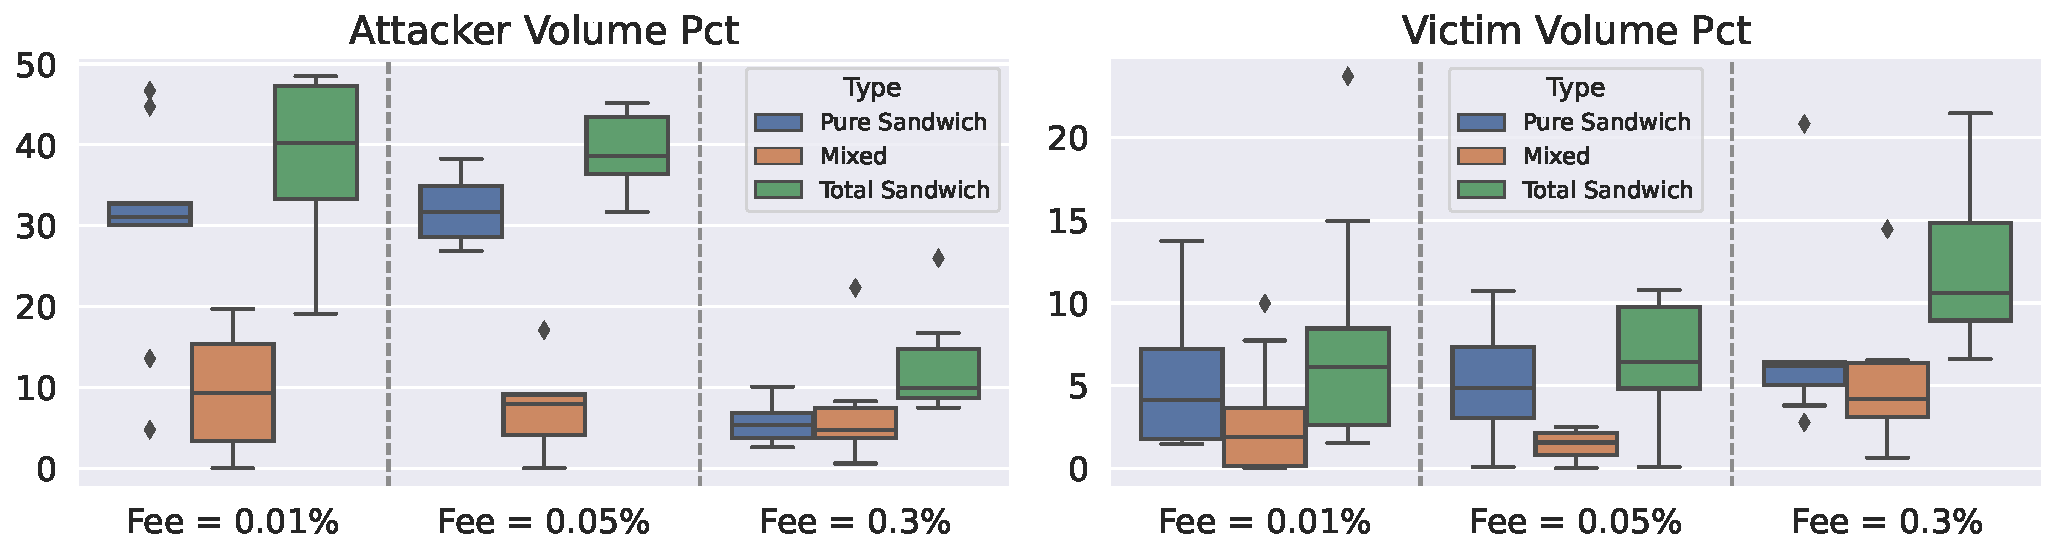
\includegraphics[height=0.17\linewidth]{figures_st_app/sand_impact_x_paper.pdf}
% \caption{Impact of sandwich attacks on trading volumes. The left plot shows the percentage of total volume linked to sandwich swaps (front-run and back-run), while the right plot presents the percentage volume from victim swaps. Blue boxes denote pure sandwich attacks, orange boxes indicate mixed attacks, and green boxes combine both categories. Pools are grouped according to fee tiers.}
% \label{fig:sand_impact_x_paper}
% \end{figure}

% Regarding attacker identities, approximately 64\% of pure sandwich attacks were executed by the wallet "jaredfromsubway." Additionally, 5, 8, and 24 wallets contributed at least 2\%, 1\%, and 0.5\% of total attacks, respectively.






\bibliographystyle{abbrv}
\bibliography{bibliography}
\end{document}
